\documentclass[11pt,b5paper,oneside,final]{book}

\usepackage[utf8]{inputenc}
\usepackage{changepage}
\usepackage{titlesec}
\usepackage[pdfencoding=auto, psdextra]{hyperref}
\usepackage{amsmath}
\usepackage[a4paper]{geometry}
\usepackage{float}
\usepackage{longtable}
\usepackage{cite}
\usepackage{subcaption} % proper subcaptions
\usepackage{cleveref} % proper referencing of subcaptions
\usepackage[all]{nowidow}
\usepackage{pdfpages}
%\usepackage[sectionbib]{chapterbib}


% bibliography
\bibliographystyle{cj}

% margin
\newgeometry{left=3.4cm,right=2.5cm,top=2.5cm,bottom=2.5cm}

% graphics
\usepackage{graphicx}
\graphicspath{{figures/},{logos/},{articles/}}

% fonts
\usepackage{sansmath}
\usepackage{mathpazo}
%\usepackage{tgheros}
\usepackage[light]{CrimsonPro}

% colors
\usepackage{color}
\usepackage{xcolor}
\definecolor{green}{HTML}{16A53F}
\definecolor{blue}{HTML}{0A59B8}
% heading setting
\titleformat{\chapter}[display]
  {\sffamily\bfseries\Huge\center}
  {\thechapter}
  {1ex}
  {\titlerule\vspace{1.5ex}}
  []
\titleformat*{\section}{\LARGE\bfseries\sffamily}
\titleformat*{\subsection}{\Large\bfseries\sffamily}
\titleformat*{\subsubsection}{\large\bfseries\sffamily}

% TOC
\setcounter{tocdepth}{3}
\setcounter{secnumdepth}{3}

% appendix
%\newcommand{\setappendix}{Appendix~\thechapter:~}
%\newcommand{\setchapter}{\thechapter~}
%\titleformat{\chapter}{\bfseries\LARGE}{%
%  \ifnum\pdfstrcmp{\@currenvir}{appendices}=0
%    \setappendix
%  \else
%    \setchapter
%  \fi}{0em}{}
%\usepackage[titletoc]{appendix}

% newcommands
\newcommand{\AAA}{\textup\AA{ }}
\newcommand{\pka}{p$K_\mathrm{a}$ }
\newcommand{\pkaa}{p$K_\mathrm{a}$}
\usepackage{calc}
\newlength{\depthofsumsign}
\setlength{\depthofsumsign}{\depthof{$\sum$}}
\newlength{\totalheightofsumsign}
\newlength{\heightanddepthofargument}
\newcommand{\nsum}[1][1.4]{% only for \displaystyle
    \mathop{%
        \raisebox
            {-#1\depthofsumsign+1\depthofsumsign}
            {\scalebox
                {#1}
                {$\displaystyle\sum$}%
            }
    }
}

\begin{document}

\include{todo}

\pagenumbering{roman}
\pagestyle{empty}

%\pdfbookmark{Tituln{\'{i}} strana}{Titulni strana}


% booklet page
\vspace*{3mm}

\includegraphics[width=10cm]{muni-lg-eng-black} 

%{\fontsize{28pt}{28pt}\selectfont{\textbf{MASARYK UNIVERSITY}}}\\[2mm]
\hspace{6mm}{\fontfamily{qhv}\fontsize{26pt}{28pt}\selectfont{\textbf{Faculty of Science}}}\\[1mm] %textsc
\vspace{6cm}

\hspace{6mm}{\fontfamily{qhv}\fontsize{28pt}{26pt}\selectfont{Doctoral Thesis}}\\

%\vspace*{9mm}

\vfill


\hspace{6mm}{\fontfamily{qhv}\fontsize{20pt}{20pt}\selectfont{Stanislav Geidl}}

\vspace{1cm}

\hspace{6mm}{\fontfamily{qhv}\fontsize{20pt}{20pt}\selectfont{Brno 2021}}
\clearpage

\vspace*{3mm}

\includegraphics[width=10cm]{muni-lg-eng-black} 

%{\fontsize{28pt}{28pt}\selectfont{\textbf{MASARYK UNIVERSITY}}}\\[2mm]
\hspace{6mm}{\fontfamily{qhv}\fontsize{26pt}{28pt}\selectfont{\textbf{Faculty of Science}}}\\[1mm] %textsc


\hspace{6mm}{\fontfamily{qhv}\fontsize{14pt}{28pt}\selectfont{\textbf{National Centre for Biomolecular Research}}}\\[1mm] %textsc

\vspace{2.2cm}

\hspace{4.5mm}{\fontfamily{qhv}\fontsize{26pt}{30pt}\selectfont{
  \parbox{\textwidth}{Chemoinformatical \\
    Methods for Prediction \\
    of Physico-Chemical \\
    Properties of Molecules}
}}

\vspace{5mm}

\hspace{6mm}{\fontfamily{qhv}\fontsize{16pt}{16pt}\selectfont{Doctoral Thesis}}

\vspace{1cm}

\hspace{6mm}{\fontfamily{qhv}\fontsize{24pt}{26pt}\selectfont{Stanislav Geidl}}

\vfill

\hspace{6mm}{\fontfamily{qhv}\fontsize{14pt}{14pt}\selectfont{
  Supervisor: doc. RNDr. Radka Svobodová, Ph.D. 
}}

\vspace{1cm}

\hspace{7mm}{\fontfamily{qhv}\fontsize{20pt}{20pt}\selectfont{Brno 2021}}
\normalsize
\clearpage

%\restoregeometry
%\newgeometry{left=3.6cm,right=3.6cm}
%\pagestyle{empty}
\begin{center}
\vspace*{9cm}
  \textsc{To my grandma.}

  \textsc{In memory of my grandpa and profesor Koča.}
\end{center}
\normalsize
\clearpage

\vfill
\section*{Bibliografický záznam}
\def\arraystretch{1.5}
\begin{tabular}{ lp{7.5cm} } 
  \textbf{Autor:}            & RNDr. Stanislav Geidl \\
                             & Přírodovědecká fakulta, Masarykova univerzita \\
                             & Národní centrum pro výzkum biomolekul \\
  \textbf{Název práce:}      & Chemoinformatické metody predikce \\
                             & fyzikálně-chemických vlastností molekul \\
  \textbf{Studijní program:} & Biomolekulární chemie a bioinformatika \\
  \textbf{Vedoucí práce:}    & doc. RNDr. Radka Svobodová, Ph.D. \\
  \textbf{Konzultant práce:} & prof. RNDr. Jaroslav Koča, DrSc. \\
  \textbf{Akademický rok:}   & 2020/2021 \\
  \textbf{Počet stran:}      & xii\,$+$\,89\\
  \textbf{Klíčová slova:}    & \input{keywords_cz.txt} \\
\end{tabular}
\normalsize
\clearpage

\vfill
\section*{Bibliographic Entry}
\def\arraystretch{1.5}
\begin{tabular}{ lp{7.5cm} } 
  \textbf{Author:}                & RNDr. Stanislav Geidl \\
                                  & Faculty of Science, Masaryk University \\
                                  & National Centre for Biomolecular Research \\
  \textbf{Title of Thesis:}       & Chemoinformatical Methods for Prediction \\
                                  & of Physico-Chemical Properties of Molecules \\ 
  \textbf{Degree Programme:}      & Biomolecular chemistry and bioinformatics \\
  \textbf{Supervisor:}            & doc. RNDr. Radka Svobodová, Ph.D. \\
  \textbf{Supervisor Specialist:} & prof. RNDr. Jaroslav Koča, DrSc. \\
  \textbf{Academic Year:}         & 2020/2021 \\
  \textbf{Number of Pages:}       & xii\,$+$\,89\\
  \textbf{Keywords:}              & \input{keywords_en.txt} \\
\end{tabular}
\clearpage

\pagestyle{plain}

\section*{Abstrakt}
Chemoinformatické přístupy pro výpočet fyzikálních a chemických vlastností
organických molekul, speciálně pak molekul dosud nesyntetizovaných, jsou vel\-mi
užitečné v rámci procesu vývoje léčiv a v dalších oblastech moderních pří\-ro\-dních
věd. Jednou z velmi důležitých vlastností organických molekul je disociační
konstanta (p$K_a$). p$K_a$ lze úspěšně predikovat pomocí chemoinformatických
modelů založených na parciálních atomových nábojích. Tyto modely vyžadují
molekulární 3D strukturu, kterou však lze připravit mnoha různými způsoby.

Prvním tématem, kterým jsem se v rámci své práce zabýval, je právě vliv zdroje
3D struktury molekul na přesnost predikce p$K_a$. Zjistil jsem, že výběr zdroje
3D struktury je klíčový pro úspěšnou predikci p$K_a$, přičemž 3D struktury
z databází DTP NCI a PubChem je jevily jako nejvhodnější. Z této analýzy byla
rovněž patrná nutnost kvalitních a rychle vypočítatelných parciálních atomových
nábojů, sloužících jako vstupy pro predikci p$K_a$. Uvedená oblast se stala
druhým tématem mé práce. Konkrétně jsem se zaměřil na parametrizaci metody
Electronegativity Equalization Method (EEM), sloužící pro rychlý vý\-po\-čet
parciálních atomových nábojů. Výsledkem mé práce byly EEM parametry,
poskytující kvalitní náboje pro léčiva a jim podobné organické molekuly.
Při přípravě těchto parametrů jsem si
rovněž uvědomil nutnost mít k dispozici softwarový nástroj pro výpočet nábojů a
pa\-ra\-me\-tri\-za\-ci nábojových metod. Tato problematika se stala třetím tématem mé
práce -- spo\-lu\-pra\-co\-val jsem na vývoji software NEEMP, který slouží
k parametrizaci EEM, validaci EEM parametrů a výpočtu nábojů pomocí metody EEM.

Celkově má práce poskytuje metodiky a nástroje pro stavbu kompletního workflow,
sloužícího pro výpočet p$K_a$ i u dosud nesyntetizovaných molekul. Toto workflow
zahrnuje získání 3D struktury molekul, výpočet jejich parciálních atomových
nábojů metodou EEM a využití nábojů pro predikci p$K_a$.
\clearpage

\section*{Abstract}
Chemoinformatic approaches for predicting physicochemical properties, especially
in the case of unsynthesized molecules, are beneficial in the drug design
process and other modern life science fields. One of the most important
properties of organic molecules is the dissociation constant (p$K_a$). p$K_a$ is
successfully predictable by chemoinformatics models based on partial atomic
charges -- these models require a molecules’ 3D structure that can be obtained
using different approaches. 

The first topic of my work is to analyzethe influence of 3D structure sources
on the quality of p$K_a$ prediction. I found out that the correct source
of 3D structure is crucial for p$K_a$ prediction while structures from databases
DTP NCI and PubChem appear most suitable. This work shows a need for quality and
quickly calculated charges used as input for p$K_a$ prediction. This field became
my second topic. Specifically, I focused on EEM (Electronegativity Equalization Me\-thod) for quick partial atomic charges calculation. The result of my work was
the EEM parameters, which provide high-quality charges for drug-like mo\-le\-cules.
During EEM parameters preparation, I realized a need to have a tool for partial
charge calculation and parametrization. This problem became my third topic -- I
cooperated on the development of NEEMP software that can parametrize EEM, validate
EEM parameters and calculate charges via EEM me\-thod.

Overall, my work provides a methodology and tools for building the whole
workflow used for p$K_a$ prediction, which can be used for unsynthesized
mo\-le\-cules. This workflow contains obtaining 3D structures of mo\-le\-cu\-les,
partial atomic charges calculation, and p$K_a$ prediction.

\clearpage

\vspace*{13cm}
\section*{Acknowledgements}
I want to express my deepest gratitude to my supervisors, prof. RNDr. Jaroslav
Ko\v{c}a, DrSc. and doc. RNDr. Radka Svobodov\'a, Ph.D., for their valuable
pieces of advice, support, and help during my whole
university study. I am very grateful that I had an opportunity to learn from them.
I want to thank the co-authors of all my articles and my former student for their
excellent cooperation and dedication.

I am obliged to my father, grandma, and grandpa for their push and unwavering
support. Without them, I couldn't go so far. At last but not least, I would like
to thank my partner for everything.
\clearpage

\vspace*{13cm}
\section*{Declaration}
I hereby declare that this disertation thesis is my original authorial work,
which I have worked on alone. All sources, references and literature used or
excerpted during the elaboration of this work are properly cited and listed
in a complete reference with regard to the source.

\vspace{1cm}

\begin{tabular}{p{5cm}c}
Brno, 6th September 2021  & ............................. \\
                          & Stanislav Geidl \\
\end{tabular}
\clearpage

\section*{Publication List With Definition of Autor's Contribution}

This dissertation is based on 3 articles of the dissertation author (Stanislav Geidl, SG): 

\vspace{10mm}

\underline{Geidl S}, Svobodová Vařeková R, Bendová V, Petrusek L, Ionescu C-M,
Jurka Z, Abagyan R, Koča J: \textbf{How Does the Methodology of 3D Structure
Preparation Influence the Quality of p$K_a$ Prediction?} \textit{J Chem Inf Model}
2015, \\* \textbf{55}:1088–1097.

\vspace{5mm}

SG prepared the input dataset (by extension of published datasets), performed
all the calculations, participated in the analysis of the results, and wrote
a part of the manuscript, including all tables and graphics.

\vspace{10mm}

\underline{Geidl S}, Bouchal T, Raček T, Svobodová Vařeková R, Hejret V,
Křenek A,\\* Abagyan R, Koča J: \textbf{High-quality and universal empirical atomic
charges for chemoinformatics applications.} \textit{J Cheminform} 2015,
\textbf{7}:59.

\vspace{5mm}

SG participated in the study's design, and cooperated in the preparation of
the input data (molecules and published EEM parameters) and in QM charge 
calculation. SG performed the analyses and the interpretation of the data.

\vspace{10mm}

Raček T, Pazúriková J, Svobodová Vařekova R, \underline{Geidl S}, Křenek A,
Falginella FL, Horský V, Hejret V, Koča J: \textbf{NEEMP: Software
for validation, accurate calculation and fast parameterization of EEM charges.}
\textit{J Cheminform} 2016, \textbf{8}:1.

\vspace{5mm}

SG prototyped the DE-Min approach and designed some new NEEMP features, such as
the usage of RMSE instead of $R^2$. SG also implemented a preparation of validation
reports.

\clearpage

%\pagestyle{empty}
\tableofcontents

\clearpage
\pagenumbering{arabic}


\renewcommand{\thesubfigure}{\Alph{subfigure}} % subfigure labeling a => A
% bold title of captions
\captionsetup[figure]{labelfont=bf} 
\captionsetup[subfigure]{labelfont=bf,labelformat=simple} % subfigure labeling (a) => a
\captionsetup[table]{labelfont=bf}
\captionsetup[subtable]{labelfont=bf}


\part{Introduction}

\chapter{Introduction}

In recent years, a vast amount of data about various types of molecules became
available. For example, we can obtain the complete human genome of a selected
individual in a few days, and about 150 thousand biomacromolecular structures
have been determined and published (Protein Data Bank \cite{Berman2014}).
Furthermore, more
than 100 million various small molecules are described in freely accessible
databases (e.g., Pubchem [], ZINC [], ChEMBL []). This richness of data caused
the formation of novel modern life-science research fields focused on the
utilization of this data. The best-known modern life sciences are
bioinformatics, structural bioinformatics, systems biology, genomics,
proteomics, and also chemoinformatics. These current research specializations
have provided many key results in basic and applied research (e.g. [6–12]).

One fascinating and beneficial field utilizing and processing newly available
data about small molecules (i.e., drug-like compounds) is chemoinformatics.
This discipline offers methodologies for comparing molecular similarity,
molecular database search, virtual screening, and the prediction of molecules'
properties and activities. This prediction is based on the idea that molecular
structures' similarity has a consequence -- a similarity in molecular
properties. In chemoinformatics, the structure is first described using
mathematical characteristics (so-called descriptors) -- numbers containing 3D
(or 2D or 1D) structure information and applicable as inputs of mathematical
models. Then, these models are constructed based on a relation between
descriptors and known values of the property or the activity. Such models are
called Quantitative Structure-Property Relationship (QSPR) models or
Quantitative Structure-Activity Relationship (QSAR) models.

A property, which is strongly required and is therefore often a target of
chemoinformatics prediction models is the acid dissociation constant, $K_a$,
and its negative logarithm p$K_a$. Those p$K_a$ values are of interest
in chemical, biological, environmental, and pharmaceutical research [58–60].
p$K_a$ values have found applications in many areas, such as evaluating and
optimizing drug candidate molecules, pharmacokinetics, ADME profiling,
understanding protein-ligand interactions, etc. Moreover, the critical
physicochemical properties such as permeability, lipophilicity, solubility,
etc., are p$K_a$ dependent. Unfortunately, experimental p$K_a$ values are
available only for a limited set of molecules. In addition to that, obtaining
experimental p$K_a$ values for newly designed molecules is very time-consuming
because they must be synthesized first. Chemoinformatics approaches for p$K_a$
prediction are therefore currently intensively examined.

For this reason, I also focused on the chemoinformatics way of p$K_a$
prediction in my work. Very promising descriptors for p$K_a$ prediction are
partial atomic charges [] because they hold information about the distribution
of electron density within the molecule. Specifically, electron densities on
atoms close to the dissociating hydrogen provide a clue about its dissociation
ability. The most common and accurate method for calculating partial atomic
charges is an application of quantum mechanics (QM). QM calculation can be
performed via various approaches, introducing different approximation levels
(i.e., approximating a wave function by different sets of mathematical
equations, which are called basis sets). QM outputs electron distribution
in orbitals and this distribution can be divided into individual atoms using
several charge calculation schemes (e.g., MPA, NPA, AIM, Hirshfeld, MK, etc.).
Therefore, the correlation between p$K_a$ and relevant atomic charges
calculated by different QM approaches has been analyzed []. I also focused
on this file in my bachelor thesis, developed a workflow for calculation
of p$K_a$ using QM partial atomic charges and examined, which types of QM are
the most suitable [].

QM charges are accurate, but their calculation is very time-consuming. A faster
Alternative to QM charges is empirical charge calculation approaches.
Furthermore, if we would like to apply chemoinformatics p$K_a$ prediction models
practically -- for example, in pre-screening large sets of drug candidates -- we
need a fast approach. Therefore, in my master thesis, I developed a p$K_a$
prediction workflow based on charges (including Electronegativity Equalization
Method).

However, several pieces of the puzzle were still missing. For example, the
developed p$K_a$ prediction workflows [] were strongly dependent on 3D structure
source, and also, the quality of available EEM charges was low.

Therefore, my dissertation's goal was to develop a workflow that predicts p$K_a$
for molecules not synthesized yet and without available experimental 3D
structures.

Specifically, the thesis examined how to improve the process of p$K_a$
prediction via providing suitable inputs. First, the influence of 3D structure
source on p$K_a$ prediction accuracy was analyzed. Afterward, the work focused
on obtaining high-quality partial atomic charges, which served as descriptors
for p$K_a$ calculation. In the end, the authors also support the development
of methodology and software tools for obtaining these high-quality charges.

The thesis structure is the following: First, an overview of key fields is
provided (Chapter 2), i.e. -- 3D structure and approaches for its prediction,
charge calculation methods, and p$K_a$ prediction approaches. Next, the
achieved results, which we published in three research papers, are briefly
described (Chapter 3), and full-texts of the respective published papers are
attached in Part ??. During the elaboration of this thesis, I was also involved
in other projects. Most of them were not related to p$K_a$ prediction but
tightly connected to the field of chemoinformatics or structural bioinformatics.
The outcome of these projects consists of several papers and a book I have
co-authored. Their title pages are attached in Part ??.



\part{Theory and Methods}
\label{part:theory}

\chapter{Structure}

\section{Molecular Structure in Computer}

The chemical structure is the essential information for chemoinformatics and
computational chemistry calculations. We recognize different types of chemical
structures according to the complexity of information \cite{Gasteiger2006}. 

The empirical or chemical formula provides information about molecule
composition -- elements and their count. The structural formula (2D structure)
extends this information about topology -- bonds between atoms. The
three-dimensional structure also provides the conformation of a molecule -- the
relative placement of atoms in space. We try to provide conformation with the
lowest energy representing the most probable conformation of molecule
in reality. For some applications, there can even be an assembly of
these 3D structures.

In chemoinformatics, two-dimensional structures are often used, but the
three-dimensional structure can often bring new information into the
\textit{in silico} calculations or models. On the other hand, this 3D structure
can be obtained experimentally for a limited number of small molecules. What
with other molecules, including those which were not synthesized yet?

\section{3D Structure Calculation}

We apply more computationally efficient methods for 3D structure computation
because we use them as input for high-throughput methods. For this reason, many
resources were devoted to the development of fast and accurate 3D structure
prediction methods \cite{Sadowski2003}. These can be classified into the following
groups []: rule-based and data-based, fragment-based, numerical methods, and
conformational analysis. These rule-based and data-based, fragment-based
methods are partially overlying.

\subsection{Rule-Based and Data-Based Methods}

These methods [] use chemical knowledge of geometric and energetic rules known
from experiments and theoretical calculations. In these methods, we use rules
explicitly to describe, e.g., bond lengths and angles; we use data implicitly
to describe, e.g., ring conformation.

\subsection{Fragment-Based Method}

The fragment-based method [] is the incremental method using rules in the first
step to fragment a structure into parts. According to the following rules,
the parts are assembled by linking fragment templates from a library
(database). Predicted structures are created from the most similar and largest
fragments in a database as possible.

\subsection{Numerical Method}

These numerical methods [] consist of three methods: molecular mechanics
(MM), quantum mechanics, and distance geometry (DG). Distance geometry is
a great tool to prepare a reasonable initial structure, which is very close
to some low-energy conformation. For this structure, we can use
the optimization process from MM or/and QM.

\subsection{Conformational Analysis}

This method [] generates a set of conformations for one molecule using
different approaches - genetic algorithms, systematic methods, random
techniques, Monte Carlo or MD simulation. The one or more different structures
are selected based on criteria such as the number of conformers, minimum
RMSD [], only conformations with the lowest MM energy (low-energy conformers).

\chapter{Partial Atomic Charges}

\section{The Concept of Atomic Charges}

Atomic charges are a theoretical concept for the quantitative description of
electron density around every atom in a molecule. The first basic concept came
from early chemistry, where an integer expressed these charges (e.g. -1, +2).
Later, they were a real number (partial charge) in organic chemistry and
physical chemistry \cite{Atkins2011}. It is a great approach to explain the
mechanism of a lot of chemical reactions. Recently, partial atomic charges also
became popular in chemoinformatics, as they proved to be informative descriptors
for QSAR and QSPR modeling \cite{Chaves2006, Gross2002} and for other
applications \cite{Moller2005, Zhang2006, Ghafourian2000}; they can be utilized
in virtual screening \cite{Galvez1994, Stalke2011} and similarity
searches \cite{Lyne2002, Bissantz2000}. In reality, we are not able to measure
these numbers, only calculate or estimate them. For such reasons, many different
approaches for the calculation of partial atomic charges were developed.

\section{Overview of Charge Calculation Methods}

\subsection{QM Charge Methods}

These methods use a wave function as a starting point and then apply subsequent
population analysis, charge calculation scheme, or fit to some physical
observation \cite{spark}. 

Mulliken population analysis (MPA) \cite{Mulliken1955, Mulliken1955a} simply
calculates a charge of an atom as a sum of an electron density from its
molecular orbitals and a half of an electron density from its bonding orbitals.
Natural population analysis (NPA) \cite{Reed1983, Reed1985} sophisticatedly
improves the MPA method by orthogonalization of specific atoms and after this,
NPA performs charge assignment from electron density the same way as in MPA.
NPA atomic charges are more stable and independent of the size of basis sets.
Other possible population analyses are Löwdin population
analysis \cite{Lowdin1950}, Hirshfeld population analysis \cite{Hirshfeld1977}.

AIM (atoms-in-molecules) charge calculation scheme is based on the idea that
electron density measured by X-ray can help with the calculation of partial
charges. Bader and his coworkers \cite{Bader1985, Bader1991} defined an atomic
volume that is used for charge calculation. Other well-known approaches are
electrostatic potential fitting methods (ESP) like CHELPG \cite{Breneman1990}
or MK (Merz-Singh-Kollman) \cite{Besler1990} and their extension -- RESP
methods \cite{Woods2015}.

Cramer and at \cite{Marenich2009} also developed semiempirical methods -- charge
model 5 (CM5), which extends Hirshfeld population analysis by empirical
parameters to reproduce charge-dependent observables. 

\subsection{Empirical Methods}

Empirical approaches use only empirical parameters, and some of these can
calculate charges from the 3D structure or only from the topology (2D structure)
of a molecule. Therefore, they are distinctly faster than QM approaches. 

One of the first empirical methods developed, CHARGE [67], performs a breakdown
of the charge transmission by polar atoms into single-bond, double-bond, and 
triple-bond additive contributions. Other empirical methods have been developed
on the electronegativity equalization principle. One group of these empirical
approaches are using the Laplacian matrix formalism and the product is
a redistribution of electronegativity: Gasteiger-Marsili (PEOE, partial
equalization of orbital electronegativity) \cite{Cho2001, Oliferenko2006},
GDAC (geometry-dependent atomic charge) \cite{Shulga2008}, KCM (Kirchhoff charge
model) \cite{Rappe1991}, DENR (dynamic electronegativity
relaxation) \cite{Nistor2006} or TSEF (topologically symmetric energy
function) \cite{Nistor2006}.

%TODO: check that same ref for 2 methods

The second group of approaches applies the full equalization of orbital
electronegativity. For example, this group contains EEM (electronegativity
equalization method) \cite{Mortier1986} and its extensions (
ABEEM \cite{Wilmer2012}, SFKEEM \cite{Chaves2006}), QEq (charge
equilibration) \cite{Rappe1991}, EQEq (extended QEq) \cite{Wilmer2012}, or
SQE (split charge equilibration) \cite{Nistor2006}.

Group of conformationally independent methods (based on the 2D structure)
contains CHARGE, Gasteiger-Marsili, KCM, DENR, and TSEF. Group of
conformationally dependent -- geometrical charges (based on the 3D structure)
also consider an influence of conformation and includes the following methods:
GDAC, EEM, ABEEM, SFKEEM, QEq, EQeq, and SQE.

A typical representative of the topological method is the Gasteiger-Marsili
method, which first assigns charges based on atom types and then iteratively
updates atomic charges based on the closest partners. The correction is smaller
and smaller in every step until the sixth step when these corrections are too
small and atomic charges are final. Empirical parameters for this method were
calculated from QM. 

On the other hand, the EEM method needs a complete 3D structure and more
applicable charges for some of the applications.

\section{EEM Calculation}

EEM (electronegativity equalization method) \cite{Mortier1986} is one of the
most popular empirical charge calculation methods and was developed more than
twenty years ago. This method's new parameterizations [D17, D56–D62] and
extension [D59, D63, D64] are still under development. An advantage of EEM
calculation is that it considers the influence of the molecule's conformation
on the atomic charges. For this reason, EEM charges are often used
in predictive models as chemoinformatics regressors (descriptors) [D65].

EEM is based on three principles: 

The first principle is Sanderson's electronegativity equalization principle.
It assumes that the effective electronegativity of each atom in the molecule
is equal to the molecular electronegativity:

\begin{equation}
    \chi_1 = \chi_2 = \cdots = \chi_x = \bar{\chi} 
\end{equation}
where $\chi_x$ is the effective electronegativity of the atom $x$ and
$\bar{\chi}$ is the molecular electronegativity.

The second principle is the principle of the charge balance. The sum of all
charges is equal to the total charge $Q$:

\begin{equation}
    \sum_{x=1} q_x = Q
\end{equation}
where $q_x$ is the charge of the atom $x$.

And the last principle is the principle of charge-dependent electronegativity.
This principle is the definition of atomic electronegativity, and states that
the electronegativity of each atom can be expressed as a function of its charge: 

\begin{equation}
    \chi_i = A_i + B_i \cdot q_i + \kappa \sum^N_{j=1 \: i\neq{j}} \frac{q_j}{R_{i,j}} 
\end{equation}
where $R_{i,j}$ is the distance between atoms $i$ and $j$, and the coefficients
$A_i$, $B_i$ and $\kappa$ are empirical parameters. 

These principles can be summed up to a system of equations with N + 1 unknowns
(where $q_1$, $q_2$, ... , $q_N$ and $\bar{\chi}$):

\begin{equation}
    \left(
    \begin{array}{ccccc}
        B_1                    & \frac{\kappa}{R_{1,2}} & \cdots & \frac{\kappa}{R_{1,N}} & -1     \\
        \frac{\kappa}{R_{2,1}} & B_2                    & \cdots & \frac{\kappa}{R_{2,N}} & -1     \\
        \vdots                 & \ddots                 & \vdots & \vdots                 & \vdots \\
        \frac{\kappa}{R_{N,1}} & \frac{\kappa}{R_{N,2}} & \cdots & B_N                    & -1     \\ 
        1                      & 1                      & 1      & 1                      & 0      \\  
    \end{array}
    \right) \cdot
    \left(
    \begin{array}{c}
        q_1        \\
        q_2        \\
        \vdots     \\
        q_N        \\
        \bar{\chi} \\
    \end{array}
    \right) =
    \left(
    \begin{array}{c}
        -A_1   \\
        -A_2   \\
        \vdots \\
        -A_N   \\
        Q      \\
    \end{array}
    \right)
\end{equation}
The first values of parameters $A_i$ and $B_i$ were modifications
of experimental hardness and electronegativity \cite{Mortier1986}. $\kappa$ was
equal to 1. Nowadays, these parameters are calculated from the QM
charges [D17, D56–D62]. Therefore, EEM charges were correlated with the QM
charge calculated with the same method used for parametrization.

\section{Quality and Usability of EEM parameters}

The quality of EEM parameters describes how the empirical charges computed
using these EEM parameters correspond with QM charges used for EEM
parameterization. Three main characteristics can describe the quality of
EEM parameters -- the coefficient of determination [D69, D70] root mean
square error (RMSE) [D69, D70] and average absolute error ($\bar{\Delta}$).

\textbf{The coefficient of determination $R^2$} is the squared value of the
Pearson coefficient (equation \ref{eq:coef_det}). This value describes the
linear correlation rate. Values close to 1 mean that values correlate very well,
and values close to 0 mean no correlation.

\begin{equation} \label{eq:coef_det}
    R = \sqrt{\frac{
        \sum^N_{x=1}{((q^{calc}_x - \overline{q}^{calc}_x) \cdot (q^{ref}_x - \overline{q}^{ref}_x))}
    }{
        \sum^N_{x=1}{(q^{calc}_x - \overline{q}^{calc}_x)^2} \cdot \sum^N_{x=1}{(q^{ref}_x - \overline{q}^{ref}_x)^2}
    }}
\end{equation}
where $q^{ref}$ is the reference value of charge calculated by QM and $q^{calc}$
is charge value calculated by EEM. $\overline{q}^{ref}$, $\overline{q}^{calc}$
are the average value of $q^{ref}$, respectively $q^{calc}$.

\textbf{Root mean square error} RMSE is the normalized sum of squared error
describing the reliability of the model calculated by:

\begin{equation}
    \mathrm{RMSE} = \frac{
        \sum^N_{x=1}{(q^{calc}_x - q^{ref}_x)^2}
    }{
        N
    }
\end{equation}

\textbf{Average absolute error} $\overline{\Delta}$ is an averaged difference
between corresponding EEM and QM charges in a molecule and is calculated
according to an equation:

\begin{equation}
    \overline{\Delta} = \frac{
        \sum^N_{x=1}{|q^{calc}_x - q^{ref}_x|}
    }{
        N
    }
\end{equation}

Their \textbf{coverage} describes the applicability of EEM parameters.
Coverage is a percentage value describing EEM parameters' ability to calculate
charges for individual molecules in a dedicated dataset. \textit{De facto},
this coverage depends on the representation of atom types in EEM parameters.

\begin{equation}
    \mathrm{coverage} = \frac{N_{pos}}{N_{tot}}
\end{equation}
where $N_{pos}$ is the number of molecules able calculated by EEM parameters
and $N_tot$ is the total number of molecules in a dataset.

\section{EEM Parametrization}

For the parameterization of EEM charges, a lot of different methods have been
introduced []. We can summarize it into two groups: one group contains
a method that analytically solves equation x -- linear regression [] and the
second group contains optimization methods \cite{Ouyang2009}  such as
Accelerated Random Search, Particle Swarm Optimization, and Differential
Evolution algorithms. Both of these groups need input -- a set of molecules
with 3D structures and QM atomic charges. In my work, linear regression and
differential evolution were used, and therefore, they are described in more
detail below:

\textbf{The linear regression (LR)} method is based on these two equations:

\begin{equation}
    A_i + B_i \cdot x = y
\end{equation}

\begin{equation}
    \begin{array}{cc}
    x =& q_i \\
    y =& \chi_i - \kappa \sum^N_{j=1 \: i\neq{j}} \frac{q_j}{R_{i,j}} \\
    \end{array}
\end{equation}

Equations are derived from equations \ref{eq:eem1} and \ref{eq:eem2}, which
define the EEM method. In the LR method, the dataset of molecules with QM
charges can change in every iteration to improve the quality of resulting
charges. Quality criterium can be the Pearson correlation coefficient or
the coefficient of determination, and the root mean square error or different
types of errors.  An advantage of the LR method is its straightforwardness and
the possibility to optimize $\kappa$ by another iteration. On the other hand,
this method is not possible to make parametrization for some extensions of EEM
like SFKEEM and ABEEM.

\textbf{Differential Evaluation (DE)} \cite{Storn1997} is a heuristics method
to focus on finding a global minimum of a function. This method works similar
to other optimization methods -- iteratively optimize parameters to improve
the final solution. Parameters of function are set up randomly, mutated, and
evaluated until there is no best solution.

\chapter{Acid Dissociation COnstant Prediction}

\section{Motivation}

The acid dissociation constant (p$K_a$) is a physicochemical property that
characterizes the strength of acids. It is one of the essential properties
for pharmaceutical, chemical, biological and environmental research or industry.
For example, it can be used in the chemoinformatics pipeline for evaluation and
optimization of drug candidate \cite{Ishihama2002, Babic2007, Manallack2007},
ADME profiling \cite{Wan2006, Cruciani2009}, pharmacokinetics \cite{Comer2001},
understanding protein-ligand interactions \cite{Klebe2000, Lee2009}.

\section{Overview of Approaches}

Several different approaches for pKa prediction have been
developed \cite{Lee2009, Rupp2010, Fraczkiewicz2006, Ho2010}. 

\subsection{LFER (Linear Free Energy Relationships) Methods}

This is one of the oldest methods \cite{Clark1964, Perrin1981} for p$K_a$
prediction. This method uses the linear relation of Gibbs energy and p$K_a$ or
the logarithm of a reaction rate constant -- the Hammett and Taft equations.
An advantage of this method is a simple, straightforward, and quick calculation,
but on the other hand, we need substituent and reaction parameters.
This method is still used in the programs ACD/pKa \cite{acd},
EPIK \cite{Shelley2007}, and SPARC \cite{spark}.

\subsection{Database Methods}

These methods \cite{Sayle, Blower2006} use a library (database) of molecules
with known pKa values. The p$K_a$ value is taken directly from this library, or 
it is interpolated or triangulated from most similar molecules in this library.
Most accurate results are produced only for molecules that are similar to
molecules in the database. For this reason, it is essential to have
an extensive library.

\subsection{Ab Inition Quantum Mechanical Calculations}

These methods \cite{Liptak2002, Toth2001} use the fact that the dissociation 
constant can be calculated from the Gibbs energy of the reaction and from the
solvation based on equation~\ref{eq:ka}. However, there is no general approach,
and every specific calculation configuration needs to be calibrated based on
experimental values. The significant disadvantage of these methods is that they
are time-consuming. On the other hand, these methods can be very accurate if
they use correct calibration parameters. It is only one of the few methods that
can be used to extend the training dataset with experimental values or validate
some of this experimental value. It means that other methods can be improved
by this method. This method is implemented as a module of the Jaguar quantum
chemical software package \cite{jaguar}.

\begin{equation}
    \mathrm{p}K_a = - \log_{10} K_a
\end{equation}

\begin{equation} \label{eq:ka}
    K_a = e^{\frac{-\Delta G^\bigcirc}{RT}}
\end{equation}

% TODO: fix euler number

\subsection{QSPR Method}

The quantitative structure-property relationship method [] [] uses mainly
a linear model to describe the relationship between molecular structure and
a property of a molecule, in our case p$K_a$. In those models, structures are
presented by descriptors [] that are numerical expressions of molecular
properties. For example, descriptors can be the number of hydrogen atoms, the 
ratio between carbon atoms and all atoms in the molecule, or solvent accessible
surface area.

p$K_a$ correlates well with the polarizability, HOMO energy \cite{Gross2001},
proton-transfer energy [35],
partial atomic charges \cite{Citra1999, Gross2002, Kreye2009, Svobodova2011},
the electrostatic potential of the molecule \cite{Liu2009}, etc.
Partial atomic charges proved as very promising
descriptors \cite{Citra1999, Gross2002, Kreye2009, Svobodova2011} for p$K_a$
prediction.



\part{Results}
\label{part:results}

\chapter{Synopsis of the Results}

We published a series of articles about pKa prediction \cite{Svobodova2011, Svobodova2013} where we showed that
some specific atomic charges correlate with p$K_a$. Based on this, we were able
to build QSPR models for the prediction of this property. We also compared QM,
EEM charges, and their models.  In this dissertation, I focused only
on the last one:

\vspace{5mm}
\underline{Geidl S}, Svobodová Vařeková R, Bendová V, Petrusek L, Ionescu C-M,
Jurka Z, Abagyan R, Koča J: \textbf{How Does the Methodology of 3D Structure
Preparation Influence the Quality of p$K_a$ Prediction?} \textit{J Chem Inf Model}
2015, \textbf{55}:1088–1097.
\vspace{5mm}

In this article, we utilized different approaches to generate the 3D structures
of organic molecules. These structures were used for the building of p$K_a$
prediction models based on charge descriptors. Then we analyzed various
influences and relationships and found which methodologies for 3D structure
preparation are applicable for p$K_a$ prediction. 

We examined not only pKa prediction models employing QM charges but also the
models utilizing EEM charges. An application of EEM charges looked very
promising. Moreover, EEM charge calculation is significantly faster than
QM charge calculation. 

However, in parallel, we found one significant limitation of EEM charges -- the
parameters. It was available a reasonable number of parameter sets, but they
had only a low coverage.  For example, Bultinc's parameter
set \cite{Bultinck2002} contains parameters only for these elements: C, F, H, N,
O. This fact markedly reduced a dataset, which we were able to use for QM
charges. 

A lack of parameters disallows the usage of EEM charges in many chemoinformatics
applications. For this reason, in our follow-up work, we focused
on the development of new and more robust EEM parameters. The first step was to
develop a new parameterization tool that was easy to use and extendable.
After the prototype, we carefully prepared a new dataset of molecules, and
for this dataset, we computed EEM parameters with higher coverage. These new
parameters were published in a scientific paper:

\vspace{5mm}
\underline{Geidl S}, Bouchal T, Raček T, Svobodová Vařeková R, Hejret V,
Křenek A, Abagyan R, Koča J: \textbf{High-quality and universal empirical atomic
charges for chemoinformatics applications.} \textit{J Cheminform} 2015,
\textbf{7}:59.
\vspace{5mm}

After some tuning up and extensive research, we released and also published
the tool for EEM parametrization -- the NEEMP software:

\vspace{5mm}
Raček T, Pazúriková J, Svobodová Vařekova R, \underline{Geidl S}, Křenek A,
Falginella FL, Horský V, Hejret V, Koča J: \textbf{NEEMP: Software
for validation, accurate calculation and fast parameterization of EEM charges.}
\textit{J Cheminform} 2016, \textbf{8}:1.
\vspace{5mm}

Sections~\ref{sec:pka-article}, \ref{sec:param-article}, and
\ref{sec:neemp-article} contain a summary and \nameref{chapter:papers} full text of
all these aforementioned articles. I was also involved in other projects, and
the outcome of it is a list of additional articles and book chapters
in \nameref{chapter:publications}.

\section{How Does the Methodology of 3D Structure Preparation Influence
the Quality of pKa Prediction?} \label{sec:pka-article}

From our previous articles \cite{Svobodova2011, Svobodova2013}, we know that
the prediction of p$K_a$ is possible via QSPR models using partial atomic
charges as descriptors. The article's goal was to discover how the methodology
of 3D structure preparation influences the quality of pKa prediction.
We prepared a dataset containing 60 phenols, 82 carboxylic acids, 48 anilines,
and additional testing 53 phenols for these purposes. We took structures
from 5 different sources for all these molecules: PubChem \cite{pubchem},
DTP NCI database \cite{nci}; Balloon \cite{Vainio2007}, Frog2 \cite{frog2},
OpenBabel \cite{openbabel}, and RDKit \cite{rdkit} software. We used neutral forms of all
the molecules and dissociated forms of phenols and carboxylic acids, and
associated forms of anilines. We also optimized these structures with MM
(Molecular mechanics) and QM. All combination led to 7220 structures for that
we calculated four different QM, one semiempirical QM, four different EEM
charges, and Gasteiger-Marselli charges. We created 516 QSPR models for all
these molecules and charges. The robustness of these models was tested by
cross-validation and QM charges also by an independent test set of phenols.

We confirmed that QM and EEM charge descriptors could be used for p$K_a$
prediction. About half of all models have excellent quality with $R^2 \geq 0.9$.
We also showed that ab initio and semiempirical charges correlate with p$K_a$
and their models are very accurate. In EEM, we had models with a little worse
quality, but empirical charges are calculated much faster, and an application
in chemoinformatics is much more appropriate. In our models, we were not able
to use Gasteiger-Marsili charges to get an adequate quality. 

We focused on different types of influence. For classes of the benzene
derivates (phenols and anilines) was much easier to obtain high-quality models.
Nevertheless, for aliphatic hydrocarbon derivates (carboxylic acid), it was more
challenging.

The focus of this article was a comparison of the source of the 3D structure.
The influence of input structure for models is essential because
the result -- the quality of QSPR models -- depends on input structures and
their quality. For example, structures taken from RDKIT generated only by
distance geometry produced fragile models. On the other hand, the 3D structures
from the DTP NCI and PubChem databases, formally structures generated by CORINA
and Omega, exhibited the best performance for all the tested molecular classes
and charge calculation approaches. Structures generated by Frog2 also performed
very well. Other 3D structure sources can also be used, but with caution.

We also tried the influence of structure optimization on the quality of QSPR
models. In most cases, differences between original structures and optimized
structures were slight. 

In this article, we summed up the best workflow for the fast and accurate
prediction of pKa. This or similar workflow can also be easily applied to other
important properties for \textit{in~silico} designed molecules. Flow is about preparing
3D structures by CORINA or Omega (with no further optimization), calculation of
EEM charges for these structures, and then the EEM QSPR calculation of p$K_a$.

\subsection{My contribution}

I prepared the input dataset (by extension of published datasets), performed
all the calculations, participated in the analysis of the results, and wrote
a part of the manuscript, including all tables and graphics.

\section{High-quality and universal empirical atomic charges for
chemoinformatics applications} \label{sec:param-article}

The EEM method for charge calculation was published several decades ago.
Before our study, there were done some improvements of EEM \cite{Yang1997,
Chaves2006}, parameterizations of empirical parameters \cite{Mortier1986, Baekelandt1991, 
Bultinck2002, Bultinck2004, Chaves2006, Svobodova2007, Jirouskova2009, Ouyang2009},
and developments of new parameterization methods \cite{Svobodova2007, Bultinck2002, Chaves2006}.
However, there was a problem with the usability of EEM because the available
parameter sets had a low coverage in chemical space.    

We prepared a set of 4475 distinct small organic, drug-like molecules containing
these elements: H, C, N, O, F, P, S, Cl, Br, and I, in different functional
groups. This set was created so that each selected atom type is contained
in at least 100 molecules. CORINA calculated the 3D structure for all molecules.
The next step was the calculation of reference QM charges. We selected
6 different approaches: B3LYP/6-311G/MPA, B3LYP/6-311G/NPA, B3LYP/6-311G/AIM,
HF/6-311G/MPA, HF/6-311G/NPA, and HF/6-311G/AIM. EEM parameterization was
performed for six QM charge calculation approaches, and the whole
set of prepared molecules was used.

Our new EEM parameters get very high quality -- all coefficients of determination had
a value greater or equal to 0.9. We also showed that the used QM approach did
not prove any difference in the quality of parameters -- B3LYP and HF produced
comparable results. EEM parameters based on NPA and AIM population analysis are
slightly better than EEM parameters based on MPA.

 We also calculated coverage of our parameters previously published parameters
 on four big chemoinformatics databases of drug-like molecules — DrugBank, \cite{Law2014}
 ChEMBL, \cite{Bento2013} PubChem, \cite{pubchem} and ZINC \cite{Irwin2012}.
 We found out that their coverage is less than 60\%
 for most of the previously published parameters.  Our newly produced parameters
 showed coverage of at least 90\% for these databases. Consistency of coverage
 points out that this problem is not related to a database but concerns
 a chemical space of drug-like molecules and their atom types.

For evaluation of quality, we selected 657 approved drugs from the DrugBank
database. We compared the coefficient of determination, root mean square error
and found out that our new parameters outperform the previously published
parameters. Coverage of the old parameters on this small evaluation dataset
is like coverage on whole databases.

The quality of EEM parameters is also affected by a used QM charge scheme.
EEM parameters derived from MPA, NPA, and AIM charges showed high quality.
EEM parameters based on Hirshfeld charges were acceptable, and MK and CHELPG
charges cannot be used with EEM.  On the other hand, none of the QM theory level
and basis set combinations showed any problem in the quality of EEM parameters.
This also confirmed that we used an appropriate selection of reference QM
charges.

We also evaluated already existing tools for calculating partial atomic charges,
and all the tools showed some issues. For example, OpenBabel tool \cite{openbabel}  is using
Bult2002\_mpa parameter set \cite{Bultinck2002}, but developers extended this
set about missing atom types with parameters for different atom types. This hack
increases coverage paid by decreased EEM charges quality for molecules
containing atom type missing in the original parameter set.  

\subsection{My contribution}

I participated in the study's design, and I cooperated in the preparation of
the input data (molecules and published EEM parameters) and in QM charge 
calculation. I performed the analyses and the interpretation of the data.

\section{NEEMP: software for validation, accurate calculation, and fast
parameterization of EEM charges} \label{sec:neemp-article}

This article describes NEEMP -- a software tool with three main
functionalities -- parametrization of EEM charges from reference QM charges,
validation of EEM parameter sets (including quality and coverage calculation),
and EEM charge calculation.

NEEMP provides two different parametrization approaches:

\begin{itemize}
    \item linear regression (LE),
    \item differential evolution with the local minimization (DE-MIN) approach. 
\end{itemize}

A combination of a global optimization method with a local optimization method
improves EEM parameterization. This combined approach provides a more robust
methodology than LR. Therefore it is applicable even for heterogeneous training
sets. Specifically, we combined differential evolution (DE) \cite{Storn1997} with the local
minimization method NEWUOA \cite{Zaslavski2006}. Quality criteria for evaluation of each 
iteration of the parametrization process (both LR and DE-MIN) can be set up to
coefficient of determination ($R^2$) or the root mean square error (RMSE).

The validation mode of NEEMP calculates quality metrics, coverage, and a
graphical representation of EEM charge correlation with reference QM charges.

The calculation mode of NEEMP provides a calculation of EEM charges using an
input parameter set.

The article also presents two case studies to show the functionality and
performance of NEEMP – a parametrization and a validation case study.

The parametrization case study targets a comparison of the parameterization
method (LR vs. DE-MIN) and metrics for model validation ($R^2$ vs. RMSE).
The case study proved that LR (with both metrics) is suitable for smaller
and homogeneous datasets. DE-MIN (with RMSD metric) is a more robust approach
that can also handle the parametrization of larger and more heterogeneous
datasets. The validation case study provided similar findings to the previous
article -- low coverage of the older parameter sets. Also, a quality validation
agrees with the previous article for smaller datasets with molecules comprised
of C, H, N, and O. On the other hand, the case study uncovered an interesting
problem: in larger and more heterogeneous datasets -- the parameters set from
our previous article proved accuracy problems with some atom types. Using NEEMP,
we computed parameter sets, which are also applicable for such problematic
datasets.

\subsection{My contribution}

I prototyped the DE-Min approach and designed some new NEEMP features, such as
the usage of RMSE instead of $R^2$. I also implemented a preparation of validion
reports.

\chapter{Follow-up work and future plans}

From these results, we were able to create a tool for the calculation
of charge descriptors -- ChrgDescCalc.py \cite{Hejret2015}, and we also
successfully prepared the universal model for p$K_a$ prediction \cite{Hejret2017}.

The EEM parameters computed in our publications \cite{Geidl2015_eem, Racek2016}
became a part of AtomicChargeCalculator \cite{Ionescu2015} and also its successor 
AtomicChargeCalculator II \cite{Racek2020}.

A parameterization approach from an NEEMP article \cite{Racek2016}, was further
extended by my coworker J. Pazúriková in an article \cite{Pazurikova2016}.
A further extension of the parameterization approach
(optGM) was done by my colleague T. Raček and it allowed a parameterization
of the majority of empirical charge calculation methods (not only EEM).
An article describing optGM is now in a review process.

In the future, the development of an empirical charge calculation approach
for proteins and a parameter set fully covering Protein Data Bank is
in development.


\part{Conclusion}

\chapter{Conclusion}

The acid dissociation constant (p$K_a$) is an important property of organic
mo\-le\-cules. Its prediction (especially for unsynthesized molecules) is beneficial
in the drug design process and other modern life science fields.

Our previous articles \cite{Svobodova2011, Svobodova2013} (before my
dissertation) proved that p$K_a$ is successfully predictable by
chemoinformatics models based on partial atomic charges.

In my thesis, I focused on the first topic -- analysis of 3D structure sources
on p$K_a$ prediction. We proved that the source of the 3D structure had
a significant impact on charges and, respectively, on the quality of p$K_a$
prediction models. The models exhibited the best performance for two databases
and two software used by these databases for 3D structure generation -- 
a database DTP NCI (where CORINA generates 3D structures) and a database
PubChem (3D structures generated by Omega). Other software tools for 3D
structure generation required additional MM optimization to produce acceptable
or good p$K_a$ prediction models. In this work, we also showed that p$K_a$
prediction models had the best performance when QM or EEM charges (with specific
parameter sets) were used. Purely empirical and topological charges (e.g.,
Gasteiger-Marseli) proved as too approximated for pKa prediction. p$K_a$
prediction models based on EEM charges seemed very promising because they were
fast (no time-demanding QM charge calculation was required), and quality was
high (comparable to models based on QM charges). However, we also found that
the applicability of EEM parameters for drug-like molecules (e.g., if the
parameters cover all atomic types present in the molecule) was significantly
limited. 

It motivated us to focus on the development of EEM parameters suitable 
for p$K_a$ prediction. Specifically, we prepared a new molecule dataset and
successfully computed EEM parameter sets with more extensive coverage
for drug-like molecules and excellent quality ($R^2 > 0.9$). These newly published
parameter sets can be easily used in chemoinformatics applications
such as virtual screening or QSAR/QSPR modeling. We also prepared an OpenBabel
patch with these parameter sets.

During EEM parameters preparation, I realized a need to have a tool for partial
charge calculation and parametrization. For this reason, I focused
on the development of NEEMP software. NEEMP is the only available tool that
provides EEM parametrization, validation of EEM parameters, and calculation
of EEM charges. In NEEMP, we also included an improved parametrization process,
including the DE-MIN method that can markedly increase the quality of final
parameters for heterogeneous datasets. We published NEEMP, and in the article,
we also provided two case studies demonstrating NEEMP capabilities. The
publication also included new EEM parameters tailored for ligand molecules.

These articles together provide a solid base for preparing chemoinformatics
workflows for p$K_a$ prediction, including 3D structures and partial atomic
charges. They sum up the current state of the art and distill the
best of well-known approaches, tools, and parameters to increase the quality
of the final result.




\appendix
\setcounter{tocdepth}{3}
\setcounter{secnumdepth}{-1}

\part{Appendix}
\appendix

\addcontentsline{toc}{chapter}{Bibliography}
{\footnotesize
\bibliography{bibliography}
}

\chapter{Main papers}
\label{chapter:papers}

\clearpage

\begin{center}
\section{\centering How Does the Methodology of 3D Structure
Preparation Influence the Quality of p$K_a$ Prediction?}
    
\underline{Stanislav Geidl$^1$}, Radka Svobodová Vařeková$^{1, *}$,
Veronika Bendová$^1$, Lukáš Petrusek$^1$, Crina-Maria Ionescu$^1$,
Zdeněk Jurka$^1$, Ruben Abagyan$^2$, Jaroslav Koča$^{1, *}$

\vspace{1cm}

$^1$ National Centre for Biomolecular Research, Faculty of Science and CEITEC,
Central European Institute of Technology, Masaryk University Brno, Kamenice 5,
625 00 Brno, Czech Republic.

$^2$ Skaggs School of Pharmacy and Pharmaceutical Sciences, University of
California, 9500 Gilman Drive, San Diego, MC 0657, USA.

\vspace{1cm}

\textit{Journal of Chemical Information and  Modeling} 2015, \textbf{55}:1088–1097.

\end{center}

% 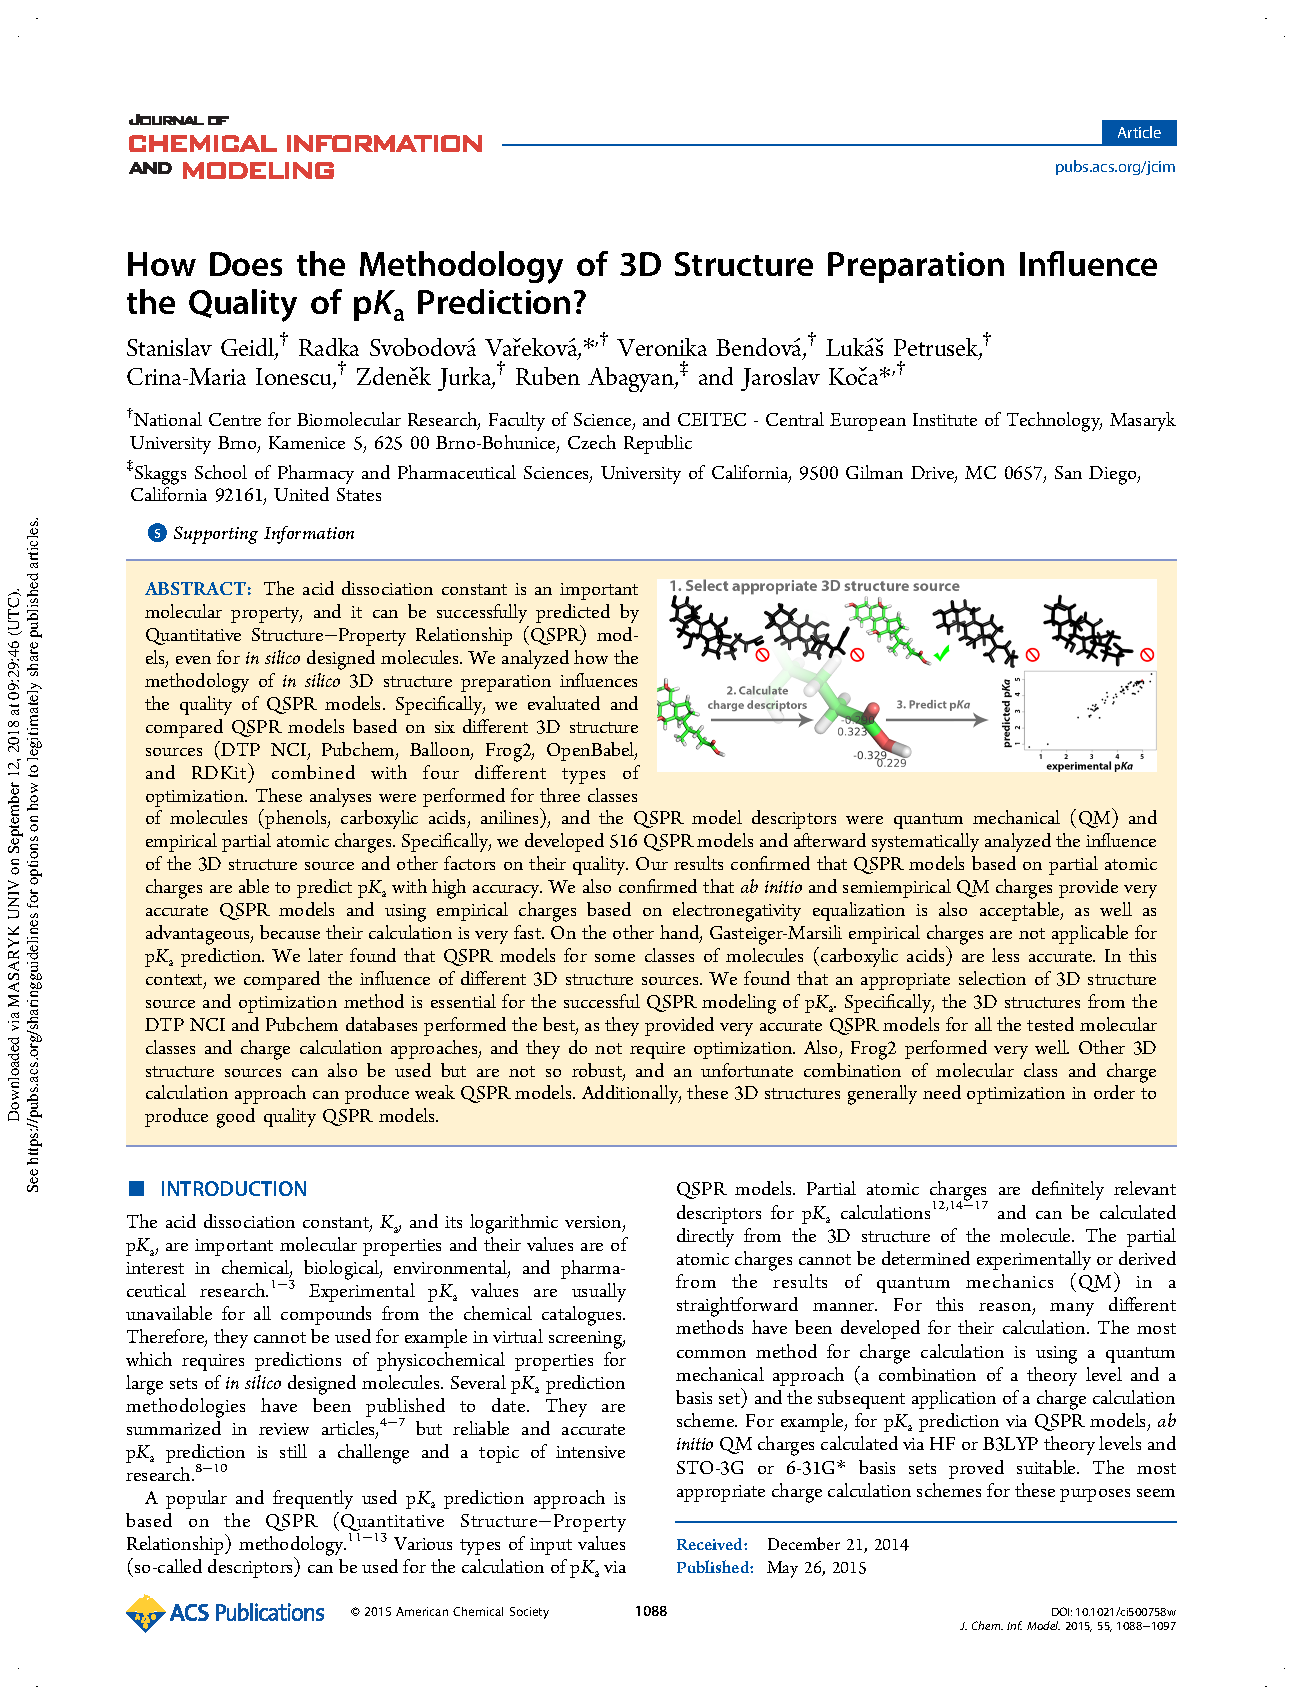
\includepdf[pages=-]{articles/pka.pdf}

%%%

\begin{center}
\section{High-quality and universal empirical atomic
charges for chemoinformatics applications}

\underline{Stanislav Geidl}$^1$, Tomáš Bouchal$^1$, Tomáš Raček$^{1,2}$,
Radka Svobodová Vařeková$^{1, *}$, Václav Hejret$^1$, Aleš Křenek$^3$,
Ruben Abagyan$^4$, Jaroslav Koča$^{1, *}$

\vspace{1cm}

$^1$ National Centre for Biomolecular Research, Faculty of Science and CEITEC,
Central European Institute of Technology, Masaryk University Brno, Kamenice 5,
625 00 Brno, Czech Republic.

$^2$ Faculty of Informatics, Masaryk University Brno, Botanická 68a, 602 00 Brno,
Czech Republic.

$^3$ Institute of Computer Science, Masaryk University Brno, Botanická 68a,
602 00 Brno, Czech Republic.

$^4$ Skaggs School of Pharmacy and Pharmaceutical Sciences, University of
California, 9500 Gilman Drive, San Diego, MC 0657, USA.

\vspace{1cm}

\textit{Journal of Cheminformatics} 2015, \textbf{7}:59.

\end{center}

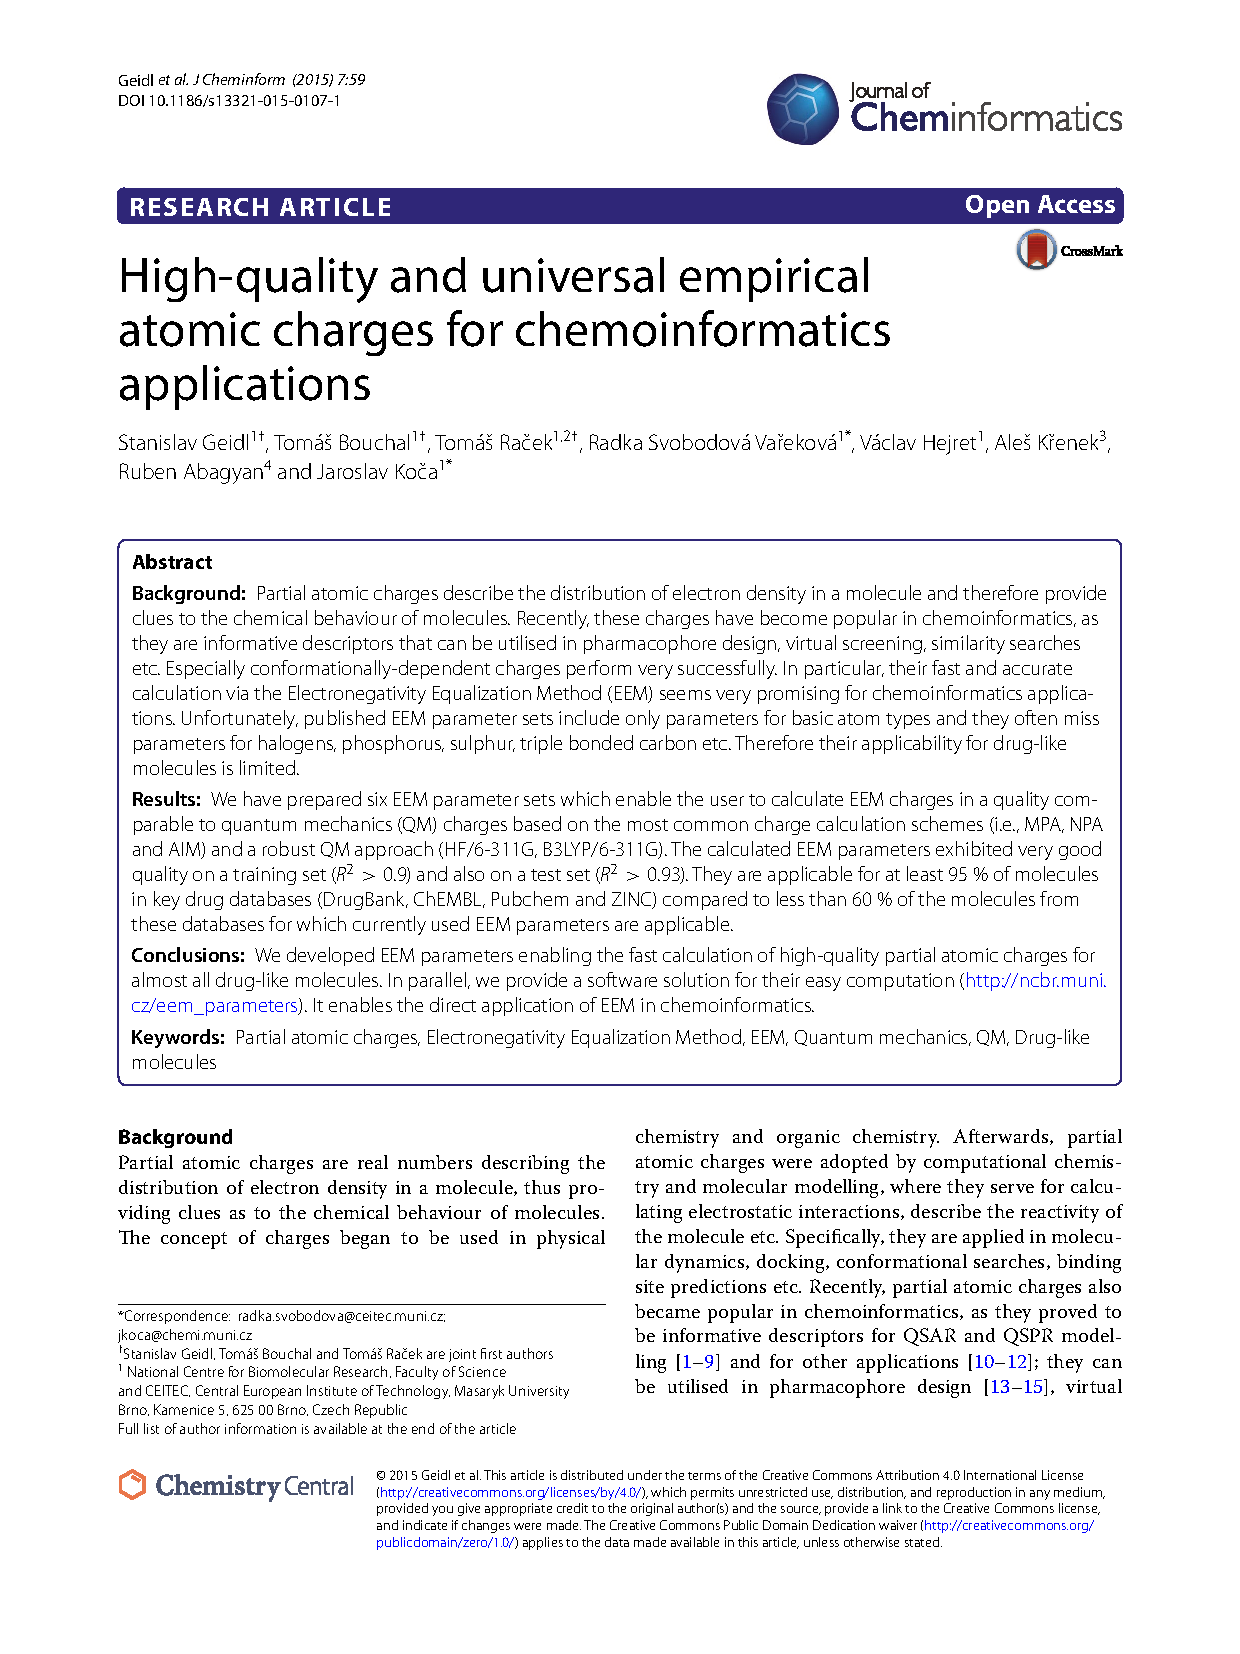
\includepdf[pages=-]{articles/eem.pdf}

%%%

\begin{center}

\section{NEEMP: Software
for validation, accurate calculation and fast parameterization of EEM charges}

Tomáš Raček$^{1,2,3}$, Jana Pazúriková$^{1,3}$, Radka Svobodová Vařekova$^{1,2,*}$,
\underline{Stanislav Geidl$^1,2$}, Aleš Křenek$^{1,2}$, Francesco Luca
Falginella$^1$, Vladimír Horský$1,3$, Václav Hejret$1$, Jaroslav Koča${1,2}$


\vspace{1cm}


$^1$ CEITEC -- Central European Institute of Technology,
Masaryk University Brno, Kamenice 5, 625 00 Brno, Czech Republic.

$^2$ National Centre for Biomolecular Research, Faculty of Science,
Masaryk University Brno, Kamenice 5, 625 00 Brno, Czech Republic.

$^3$ Faculty of Informatics, Masaryk University Brno, Botanická 68a, 602 00 Brno,
Czech Republic.

$^4$ Institute of Computer Science, Masaryk University Brno, Botanická 68a,
602 00 Brno, Czech Republic.

\vspace{1cm}

\textit{Journal of Cheminformatics} 2016, \textbf{8}:1
\end{center}

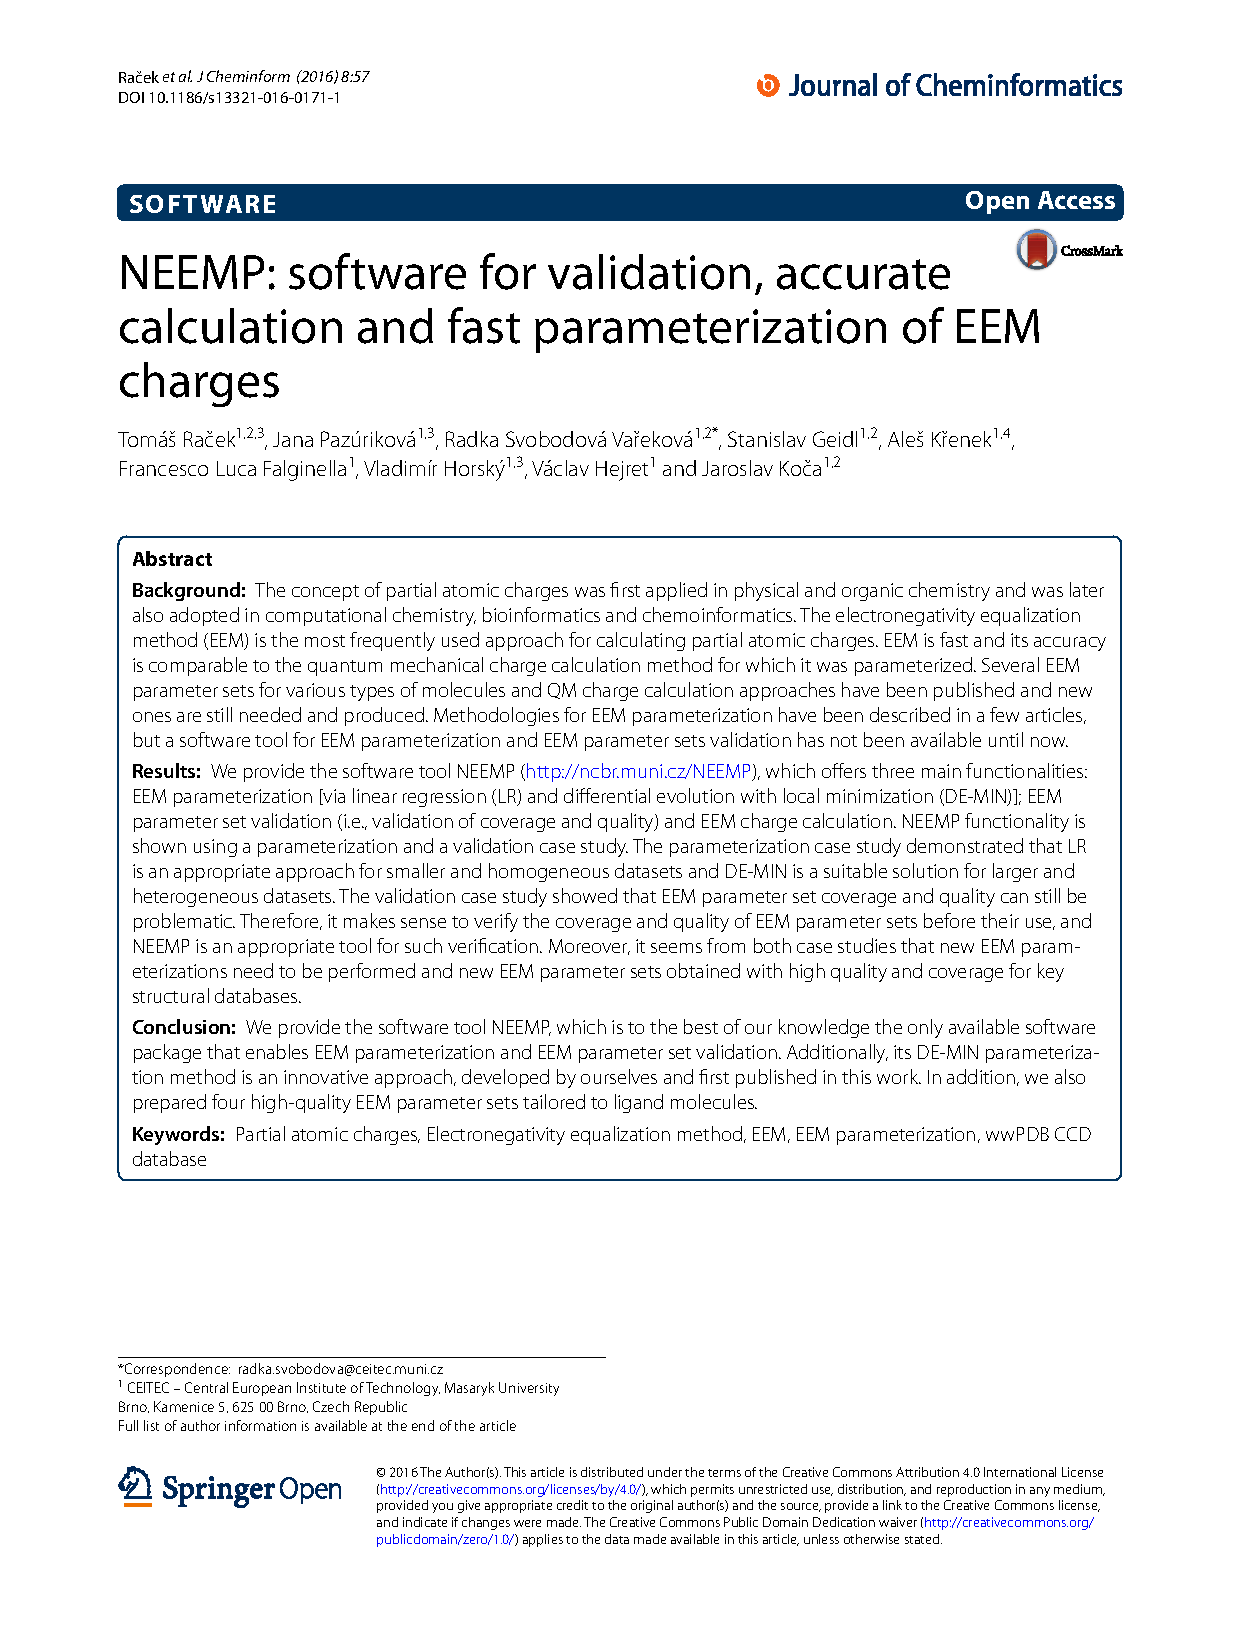
\includepdf[pages=-]{articles/neemp.pdf}

\chapter{Other Publications}
\label{chapter:publications}

This part contains the publication outcome of the projects I was collaborating
on during my PhD studies. In total there are 5 publications sorted as the list
by a year in a descending order. Further, each manuscript is represented by
its title page.

\vspace{5mm}

Koča J, Svobodová Vařeková R, Pravda L, Berka K, \underline{Geidl S}, Otyepka M:
\textbf{Structural Bioinformatics Tools for Drug Design}
\textit{Springer International Publishing, Cham} 2016.

\vspace{5mm}

Ionescu CM, Sehnal D, Falginella F L, Pant P, Pravda L, Bouchal T,
Svobodová Vařeková R, \underline{Geidl S}, Koča J: 
\textbf{AtomicChargeCalculator: Interactive Web-based calculation of atomic
charges in large biomolecular complexes and drug like molecules}
\textit{J Cheminform} 2015, \textbf{7}:50.

\vspace{5mm}

Sehnal D, Svobodová Vařeková R, Pravda L, Ionescu CM, \underline{Geidl S},
Horský V, Jaiswal D, Wimmerová M, Koča J: \textbf{ValidatorDB: database of up-to-date
validation results for ligands and non-standard residues from the Protein Data Bank}
\textit{Nucleic Acids Res} 2015, \textbf{43}:D368--D375.

\vspace{5mm}

Svobodová Vařeková R, Jaiswal D, Sehnal D, Ionescu CM, \underline{Geidl S},
Pravda L, Horský V, Wimmerová M, Koča J: \textbf{MotiveValidator: interactive
web-based validation of ligand and residue structure in biomolecular complexes}
\textit{Nucleic Acids Res} 2014, \textbf{42}:W227--W233.


\vspace{5mm}

Ionescu CM, \underline{Geidl S}, Svobodová Vařeková R,Koča J: \textbf{Rapid Calculation
of Accurate Atomic Charges for Proteins via the Electronegativity Equalization Method}
\textit{J Chem Inf Model} 2013, \textbf{53}:10.


\clearpage

%% book
\begin{center}
\section{\centering Structural Bioinformatics Tools for Drug Design}

\subsection*{\centering Extraction of Biologically Relevant Information from Structural Databases}

Jaroslav Koča$^1$, Radka Svobodová Vařeková$^1$, Lukáš Pravda$^1$,
Karel Berka$^2$, \underline{Stanislav Geidl$^1$}, David Sehnal$^1$,
Michal Otyepka$^2$

\vspace{1cm}

$^1$ National Centre for Biomolecular Research, Masaryk University Brno,
Faculty of Science National Centre Biomolecular Research, Brno-Bohunice,
Czech Republic

$^2$ Regional Centre of Advanced Technologies and Materials,
Department of Physical Chemistry, Palacký University Olomouc,
Faculty of Science Olomouc, Czech Republic

\vspace{1cm}

Book in series \textit{SpringerBriefs in Biochemistry and Molecular Biology},
published by \textit{Springer, Cham}, 2016.

\vspace{1cm}

\url{http://doi.org/10.1007/978-3-319-47388-8}

\end{center}

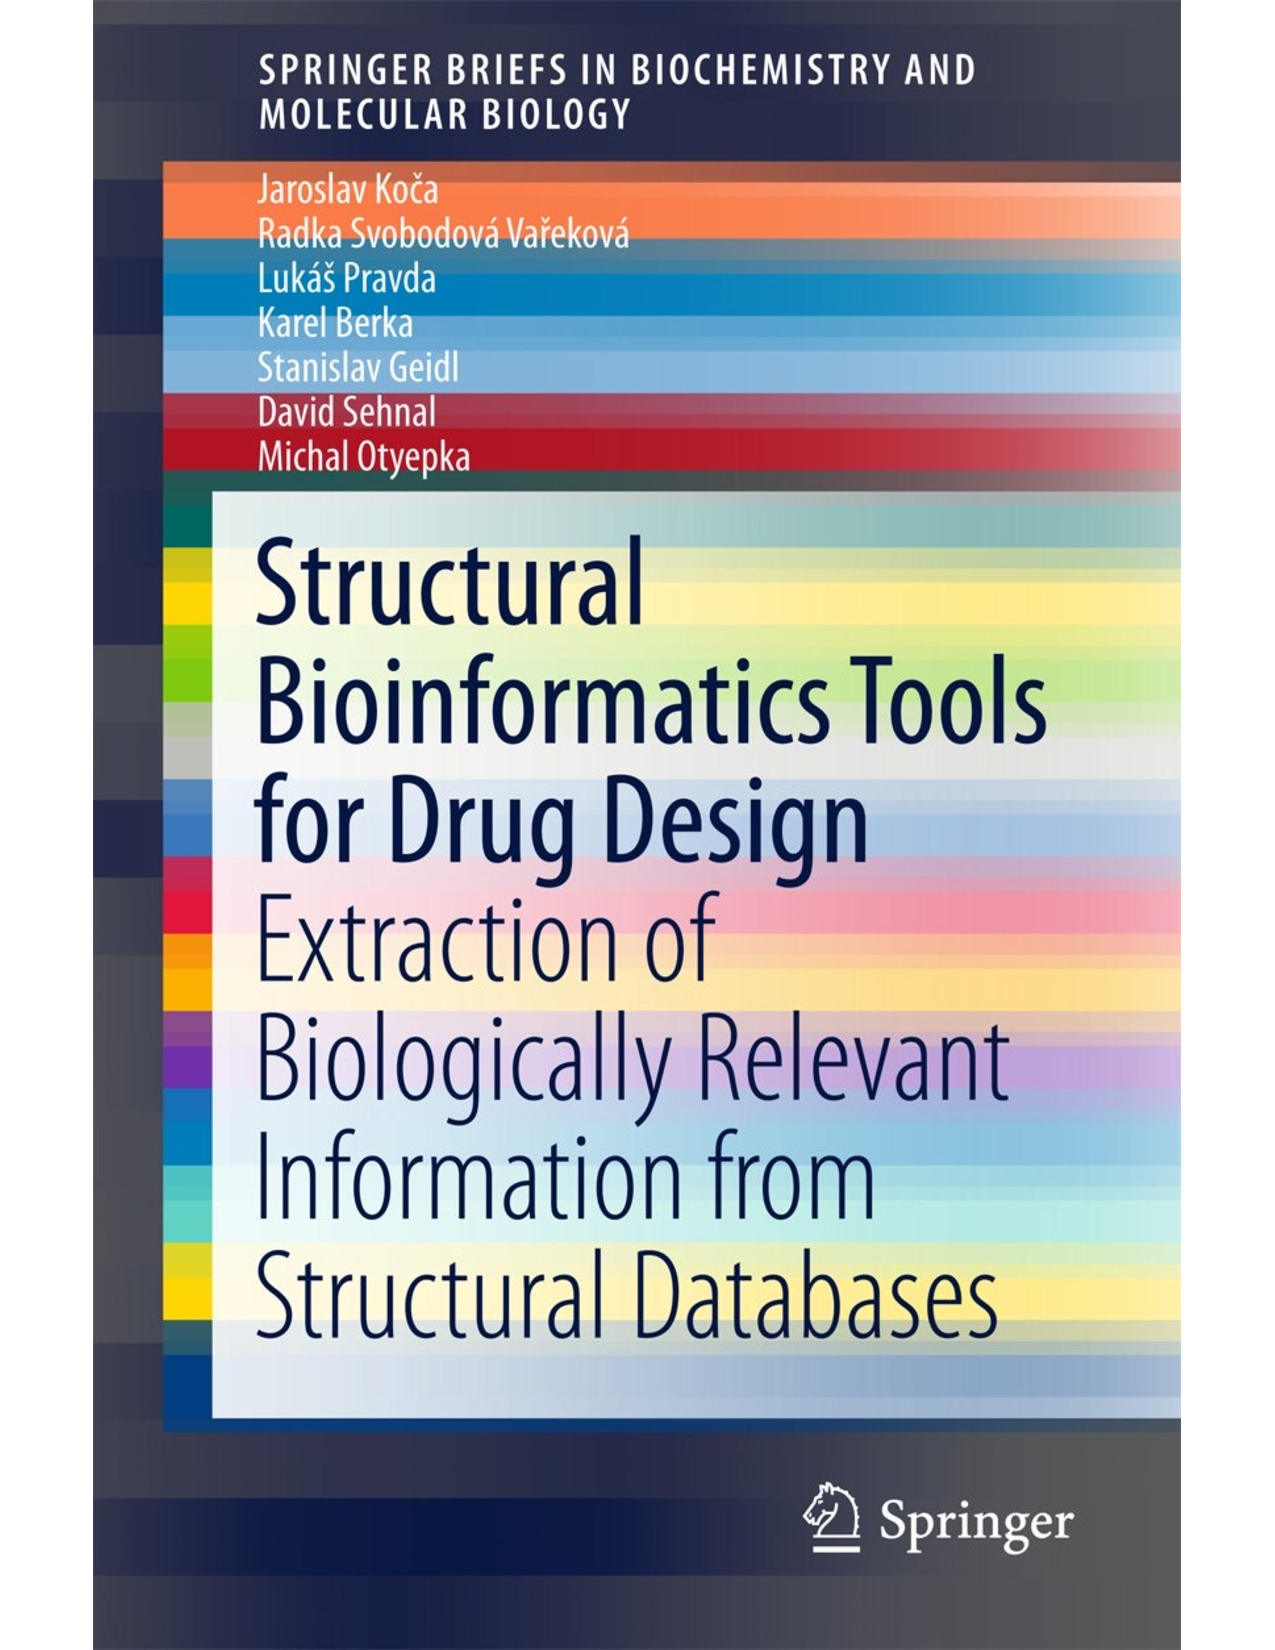
\includepdf[pages=-]{others/book.pdf}

%%% atomic charge calculator
\begin{center}
\section{\centering AtomicChargeCalculator: Interactive Web-based Calculation
of Atomic Charges in Large Biomolecular Complexes and Drug Like Molecules}

Crina-Maria Ionescu$^1$, David Sehnal$^{1, 2, 3}$, Francesco L. Falginella$^1$,
Purbaj Pant$^2$, Lukáš Pravda$^{1, 2}$, Tomáš Bouchal$^{1, 2}$,
Radka Svobodová Vařeková$^{1, 2}$, \underline{Stanislav Geidl}$^{1, 2}$,
Jaroslav Koča$^{1, 2}$

\vspace{1cm}

$^1$ CEITEC -- Central European Institute of Technology,
Masaryk University Brno, Kamenice 5, 625 00 Brno, Czech Republic.

$^2$ National Centre for Biomolecular Research, Faculty of Science,
Masaryk University Brno, Kotlářská 2, 611 37, Brno, Czech Republic.

$^3$ Faculty of Informatics, Masaryk University Brno, Botanická 68a, 602 00 Brno,
Czech Republic.

\vspace{1cm}

\textit{Journal of Cheminformatics} 2015, \textbf{7}:50.

\vspace{1cm}

\url{https://doi.org/10.1186/s13321-015-0099-x}

\end{center}

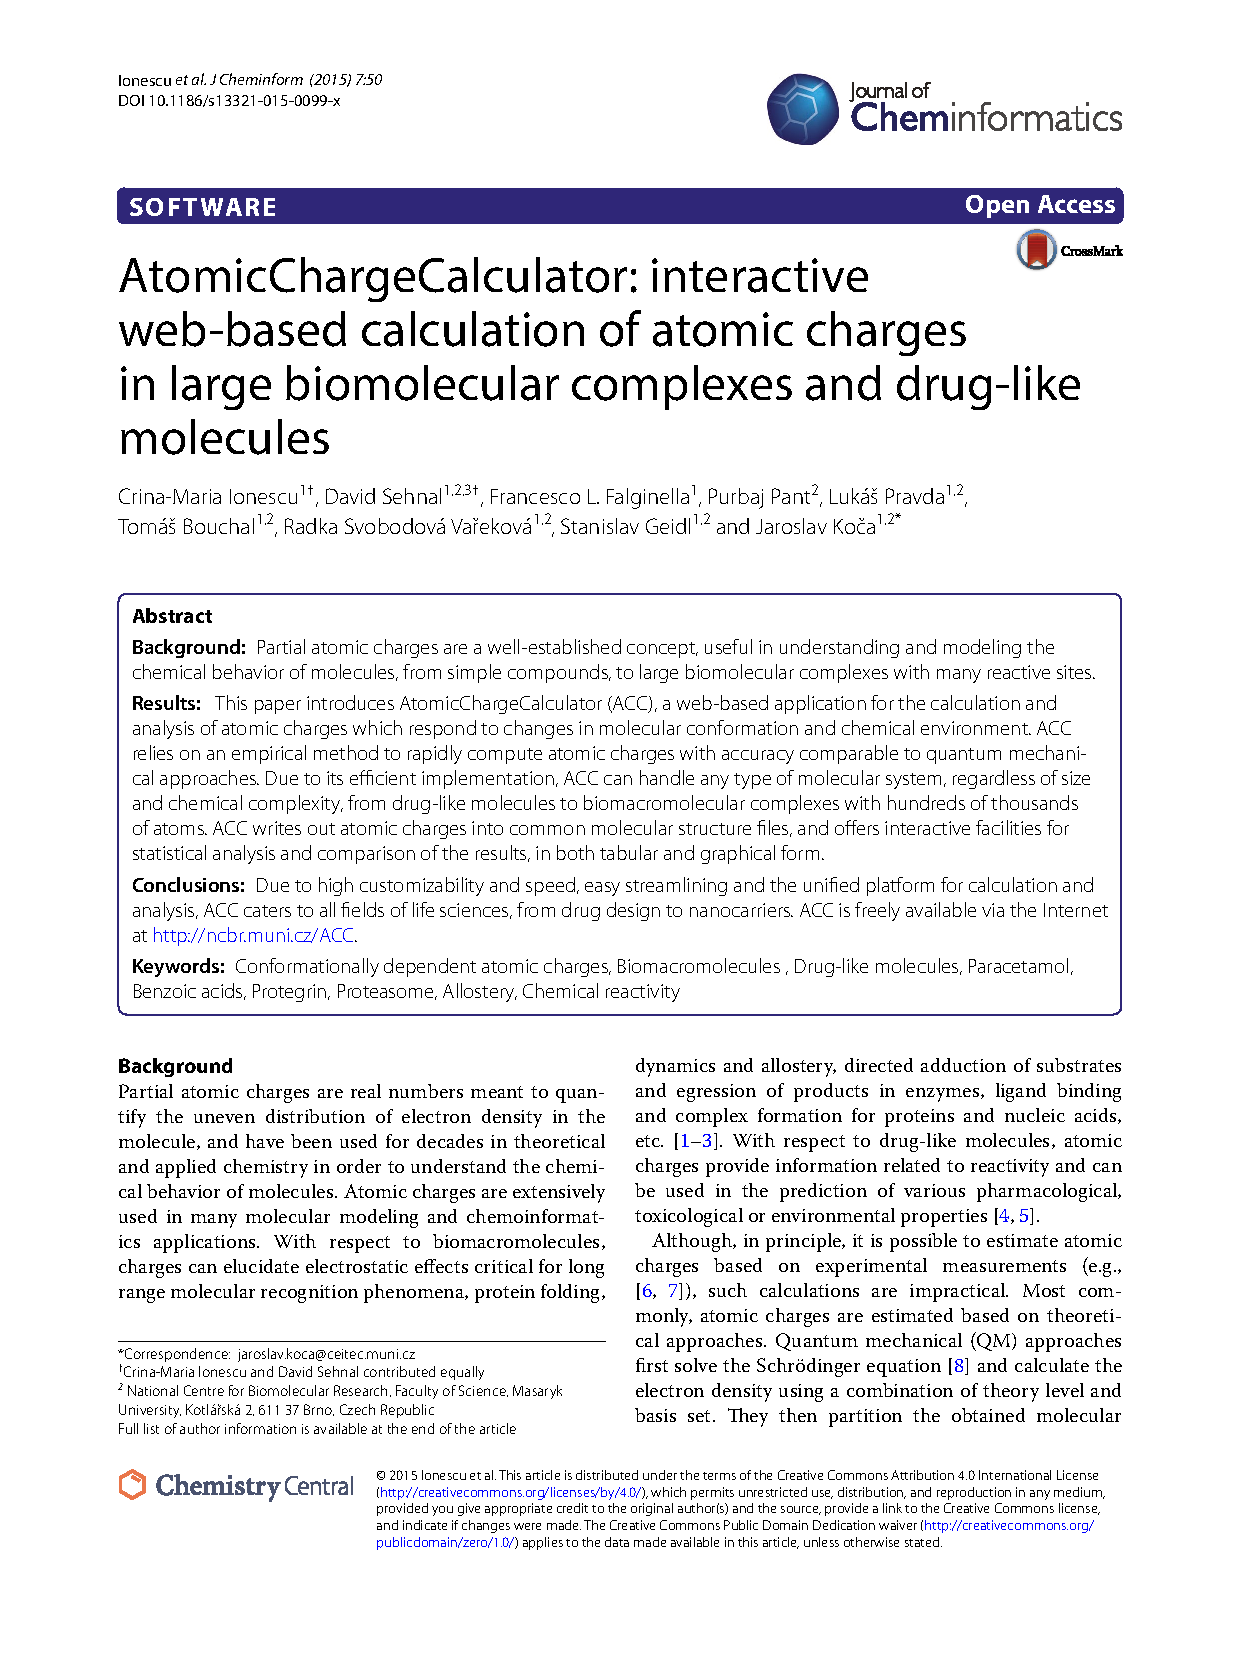
\includepdf[pages=-]{others/charge_calculator.pdf}

%%% validator DB
\begin{center}
\section{\centering ValidatorDB: Database of up-to-date
Validation Results for Ligands and Non-Standard Residues From the Protein Data Bank}

David Sehnal$^{1, 2, 3}$,
Radka Svobodová Vařeková$^{1, 2}$,
Lukáš Pravda$^{1, 2}$,
Crina-Maria Ionescu$^1$,
\underline{Stanislav Geidl}$^{1, 2}$,
Vladimír Horský$^3$,
Deepti Jaiswal$^1$,
Michaela Wimmerová$^{1, 2}$,
Jaroslav Koča$^{1, 2}$

\vspace{1cm}

$^1$ CEITEC -- Central European Institute of Technology,
Masaryk University Brno, Kamenice 5, 625 00 Brno, Czech Republic.

$^2$ National Centre for Biomolecular Research, Faculty of Science,
Masaryk University Brno, Kotlářská 2, 611 37, Brno, Czech Republic.

$^3$ Faculty of Informatics, Masaryk University Brno, Botanická 68a, 602 00 Brno,
Czech Republic.

\vspace{1cm}

\textit{Nucleic Acids Research} 2015, \textbf{43}:D368--D375.

\vspace{1cm}

\url{https://doi.org/10.1093/nar/gku1118}

\end{center}

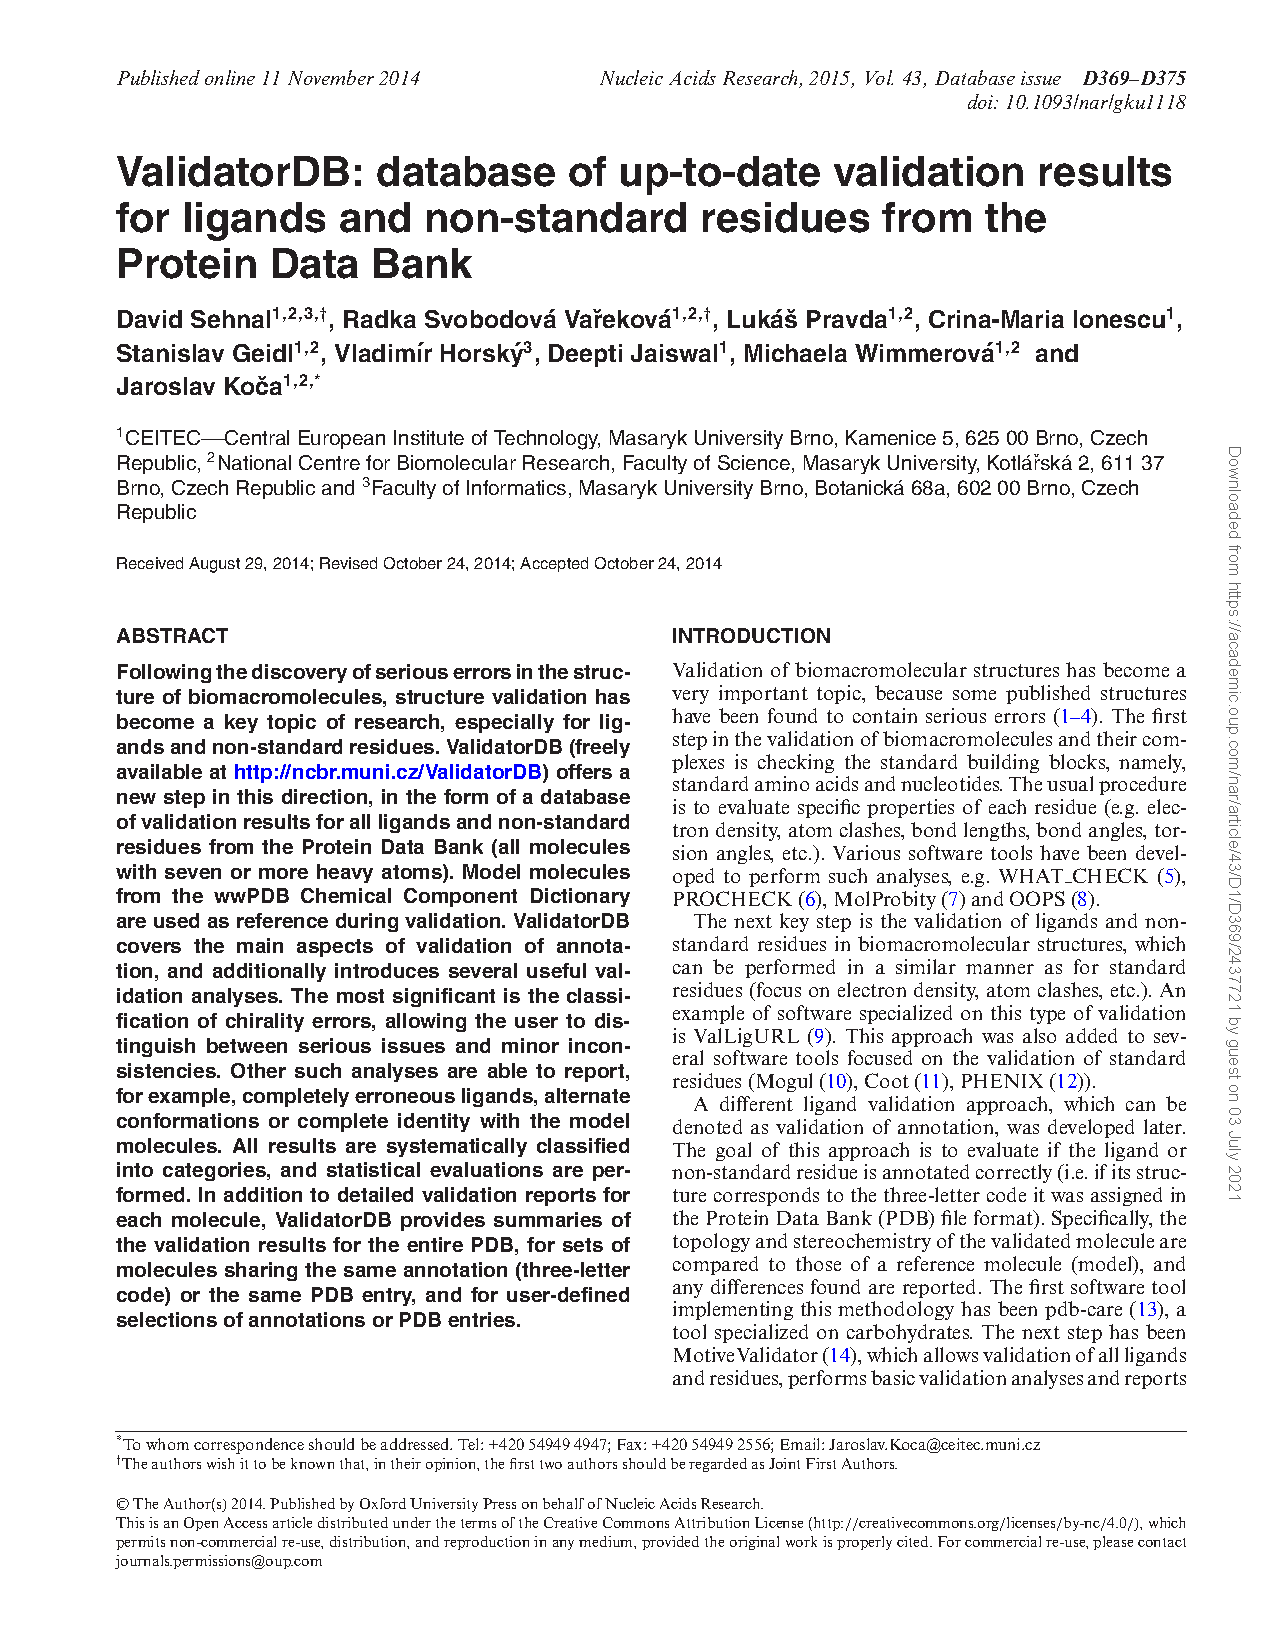
\includepdf[pages=-]{others/validator_db.pdf}

%%% motive validator
\begin{center}
\section{\centering MotiveValidator: Interactive
Web-Based Validation of Ligand and Residue Structure in Biomolecular Complexes}

Radka Svobodová Vařeková$^{1, 2}$,
Deepti Jaiswal$^1$,
David Sehnal$^{1, 2, 3}$,
Crina-Maria Ionescu$^1$,
\underline{Stanislav Geidl}$^{1, 2}$,
Lukáš Pravda$^{1, 2}$,
Vladimír Horský$^3$,
Michaela Wimmerová$^{1, 2}$,
Jaroslav Koča$^{1, 2}$

\vspace{1cm}

$^1$ CEITEC -- Central European Institute of Technology,
Masaryk University Brno, Kamenice 5, 625 00 Brno, Czech Republic.

$^2$ National Centre for Biomolecular Research, Faculty of Science,
Masaryk University Brno, Kotlářská 2, 611 37, Brno, Czech Republic.

$^3$ Faculty of Informatics, Masaryk University Brno, Botanická 68a, 602 00 Brno,
Czech Republic.

\vspace{1cm}

\textit{Nucleic Acids Research} 2015, \textbf{43}:D368--D375.

\vspace{1cm}

\url{https://doi.org/10.1093/nar/gku426}

\end{center}

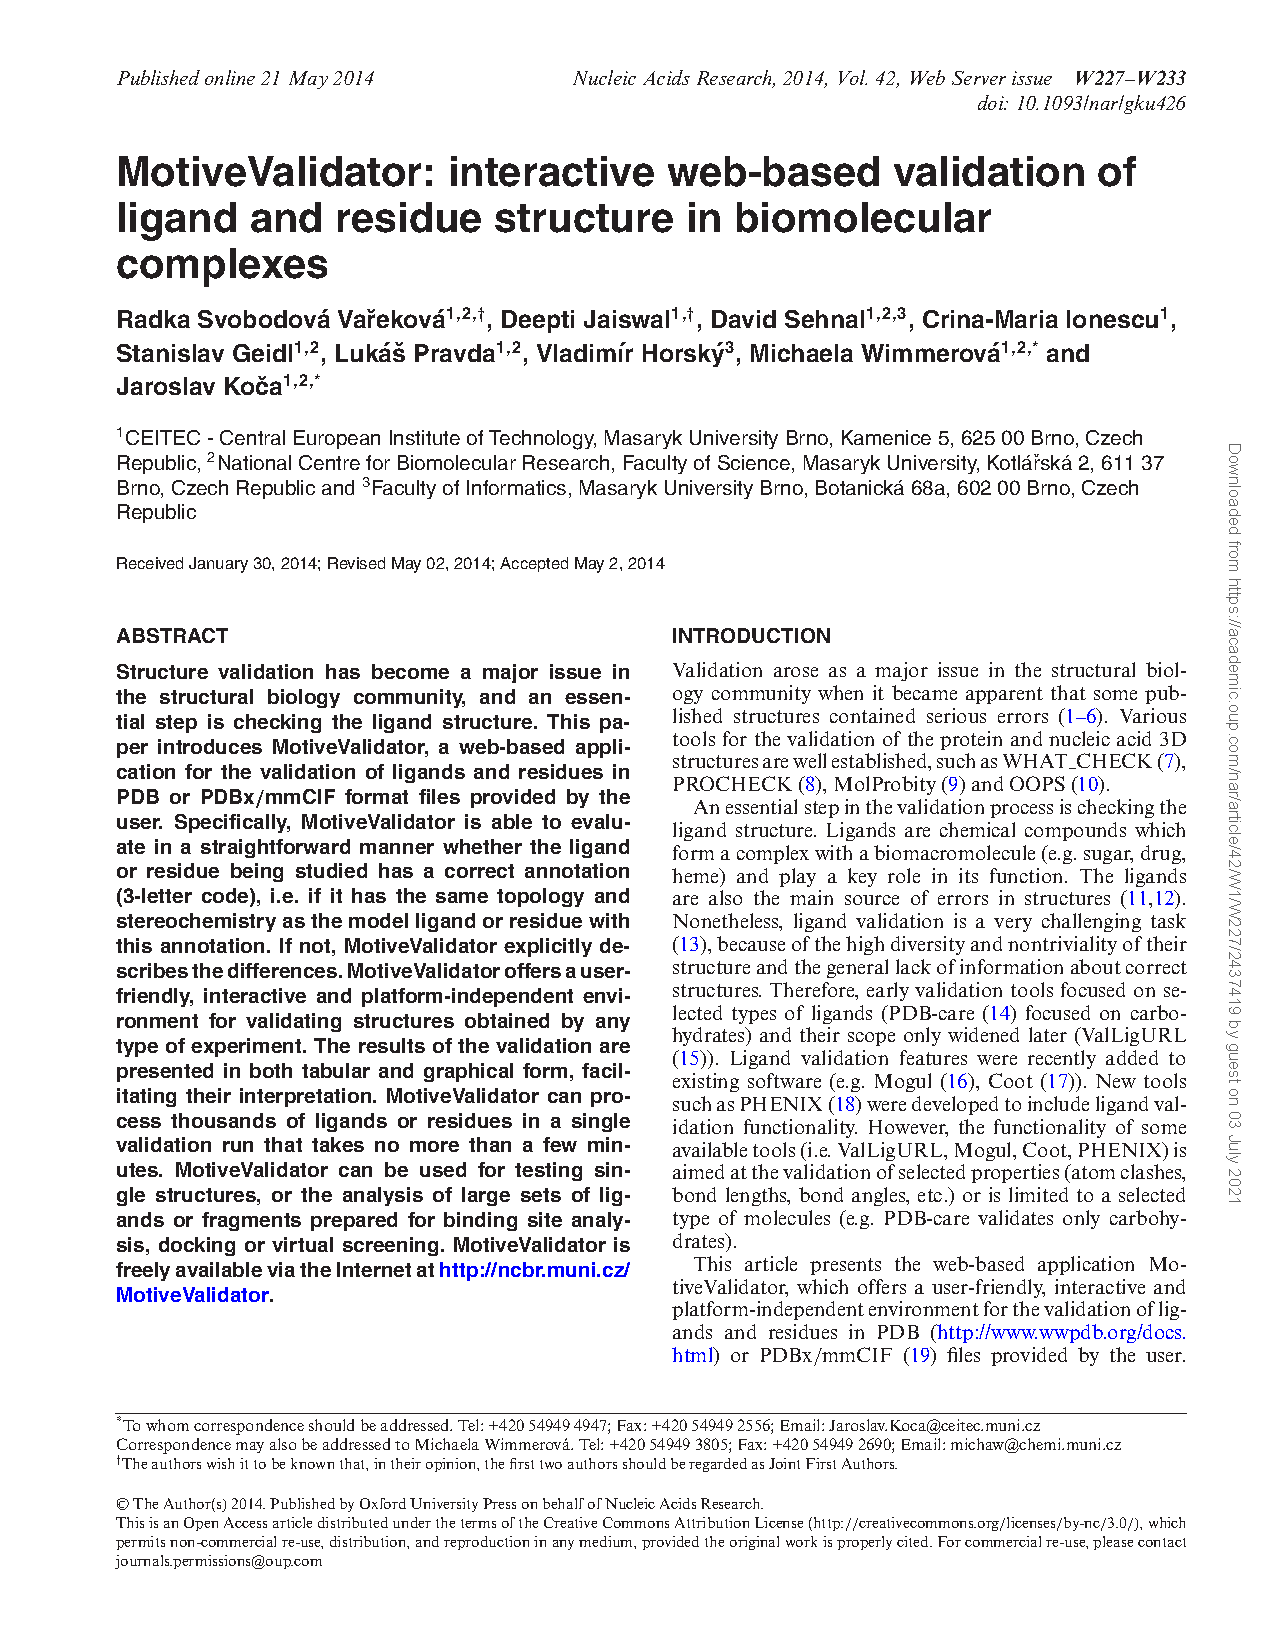
\includepdf[pages=-]{others/motive_validator.pdf}

%%% charges for proteins
\begin{center}
\section{\centering Rapid Calculation of AccurateAtomic Charges
for Proteins via the Electronegativity Equalization Method}

Crina-Maria Ionescu,
\underline{Stanislav Geidl},
Radka Svobodová Vařeková,
Jaroslav Koča

\vspace{1cm}

CEITEC--Central European Institute of Technology, and National
Centre for Biomolecular Research, Faculty of Science, Masaryk
University Brno, Kamenice 5, 625 00 Brno, Czech Republic.

\vspace{1cm}

\textit{Nucleic Acids Research} 2013, \textbf{53}:10.

\vspace{1cm}

\url{https://doi.org/10.1021/ci400448n}

\vspace{1cm}

Following page is reprinted (adapted) with permission from 
Ionescu CM, Geidl S, Svobodová Vařeková R, Koča J. Rapid calculation
of accurate atomic charges for proteins via the electronegativity
equalization method. J Chem Inf Model. 2013 Oct 28;53(10):2548-58.
doi: 10.1021/ci400448n. Epub 2013 Sep 13. PMID: 23968236.

Copyright 2015 American Chemical Society.

\end{center}

\includepdf[pages=-]{others/charges_for_proteins.pdf}
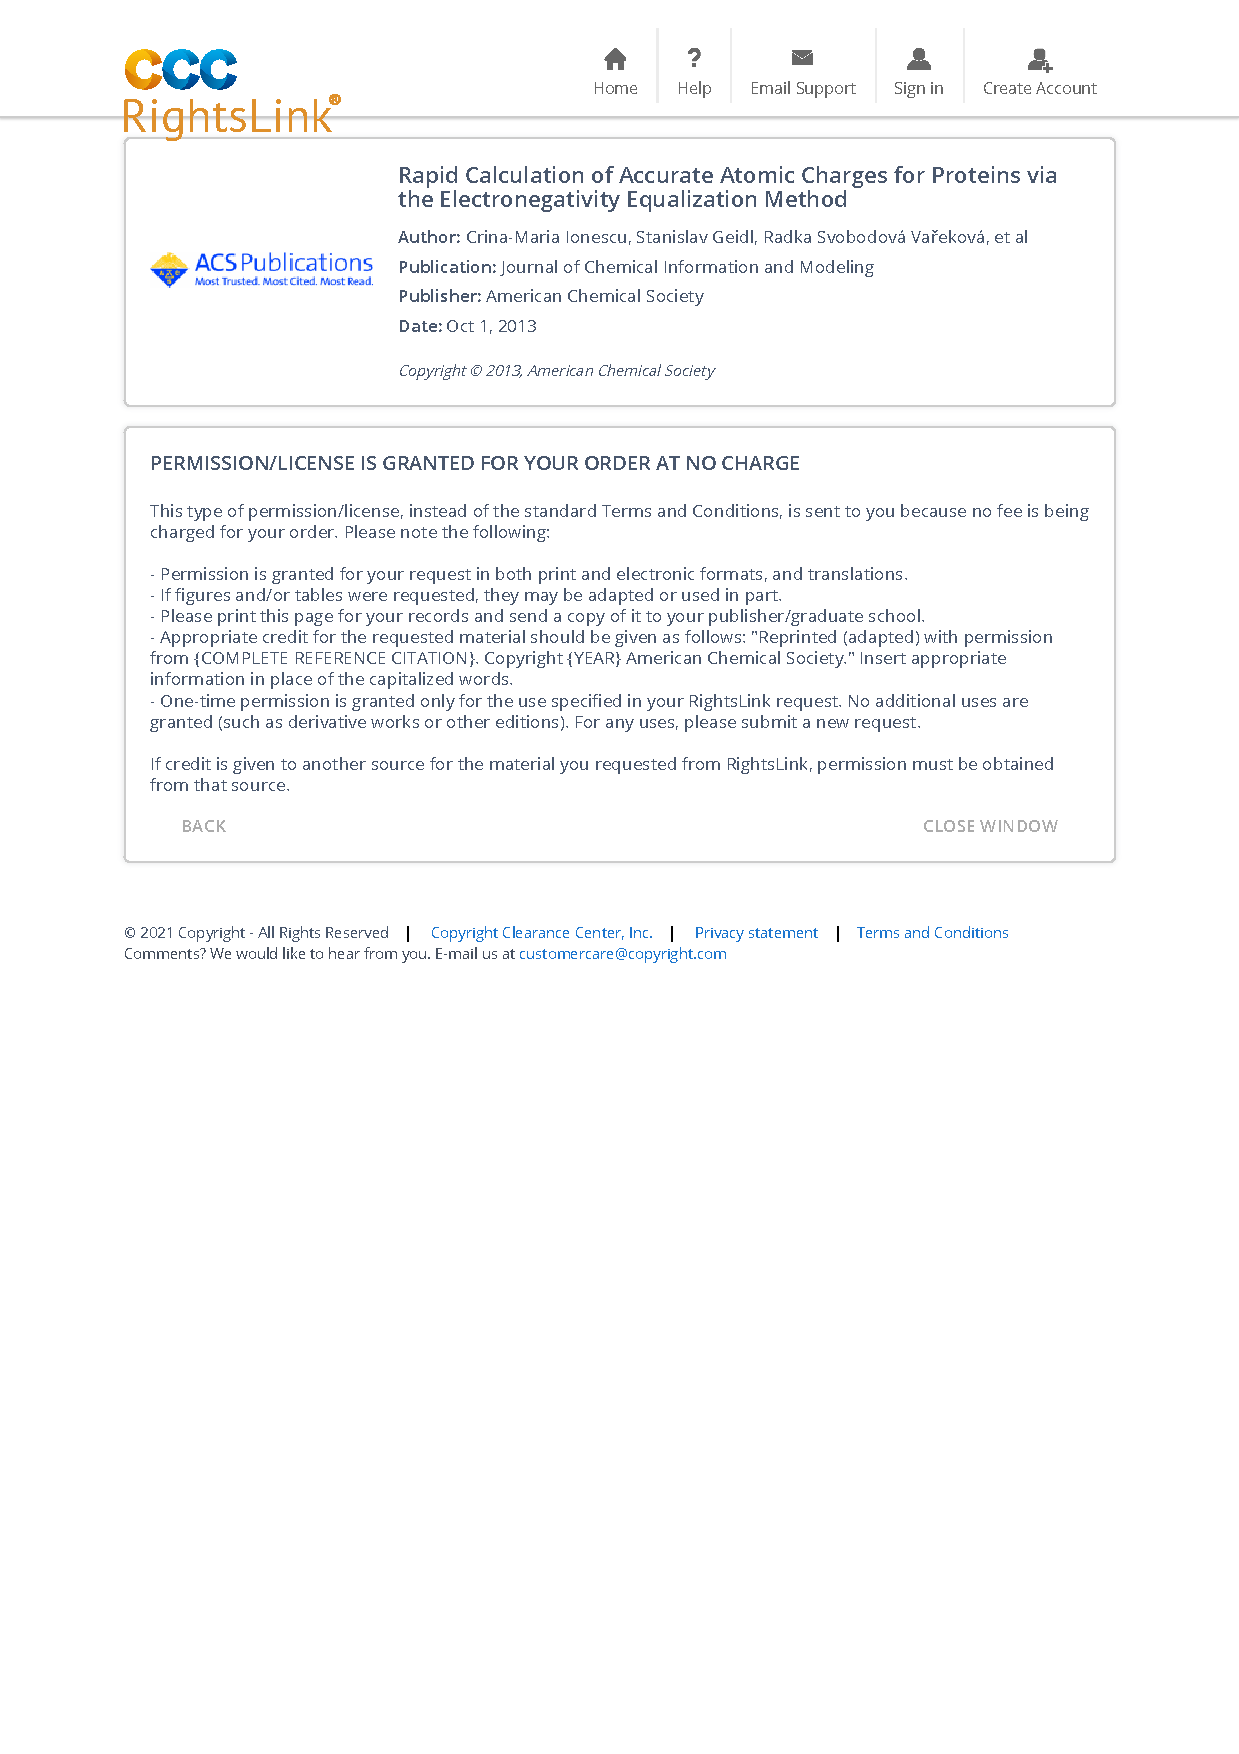
\includepdf[pages=-]{licenses/charges_for_proteins_license.pdf}


\chapter{Curriculum Vitae}
\label{chapter:cv}

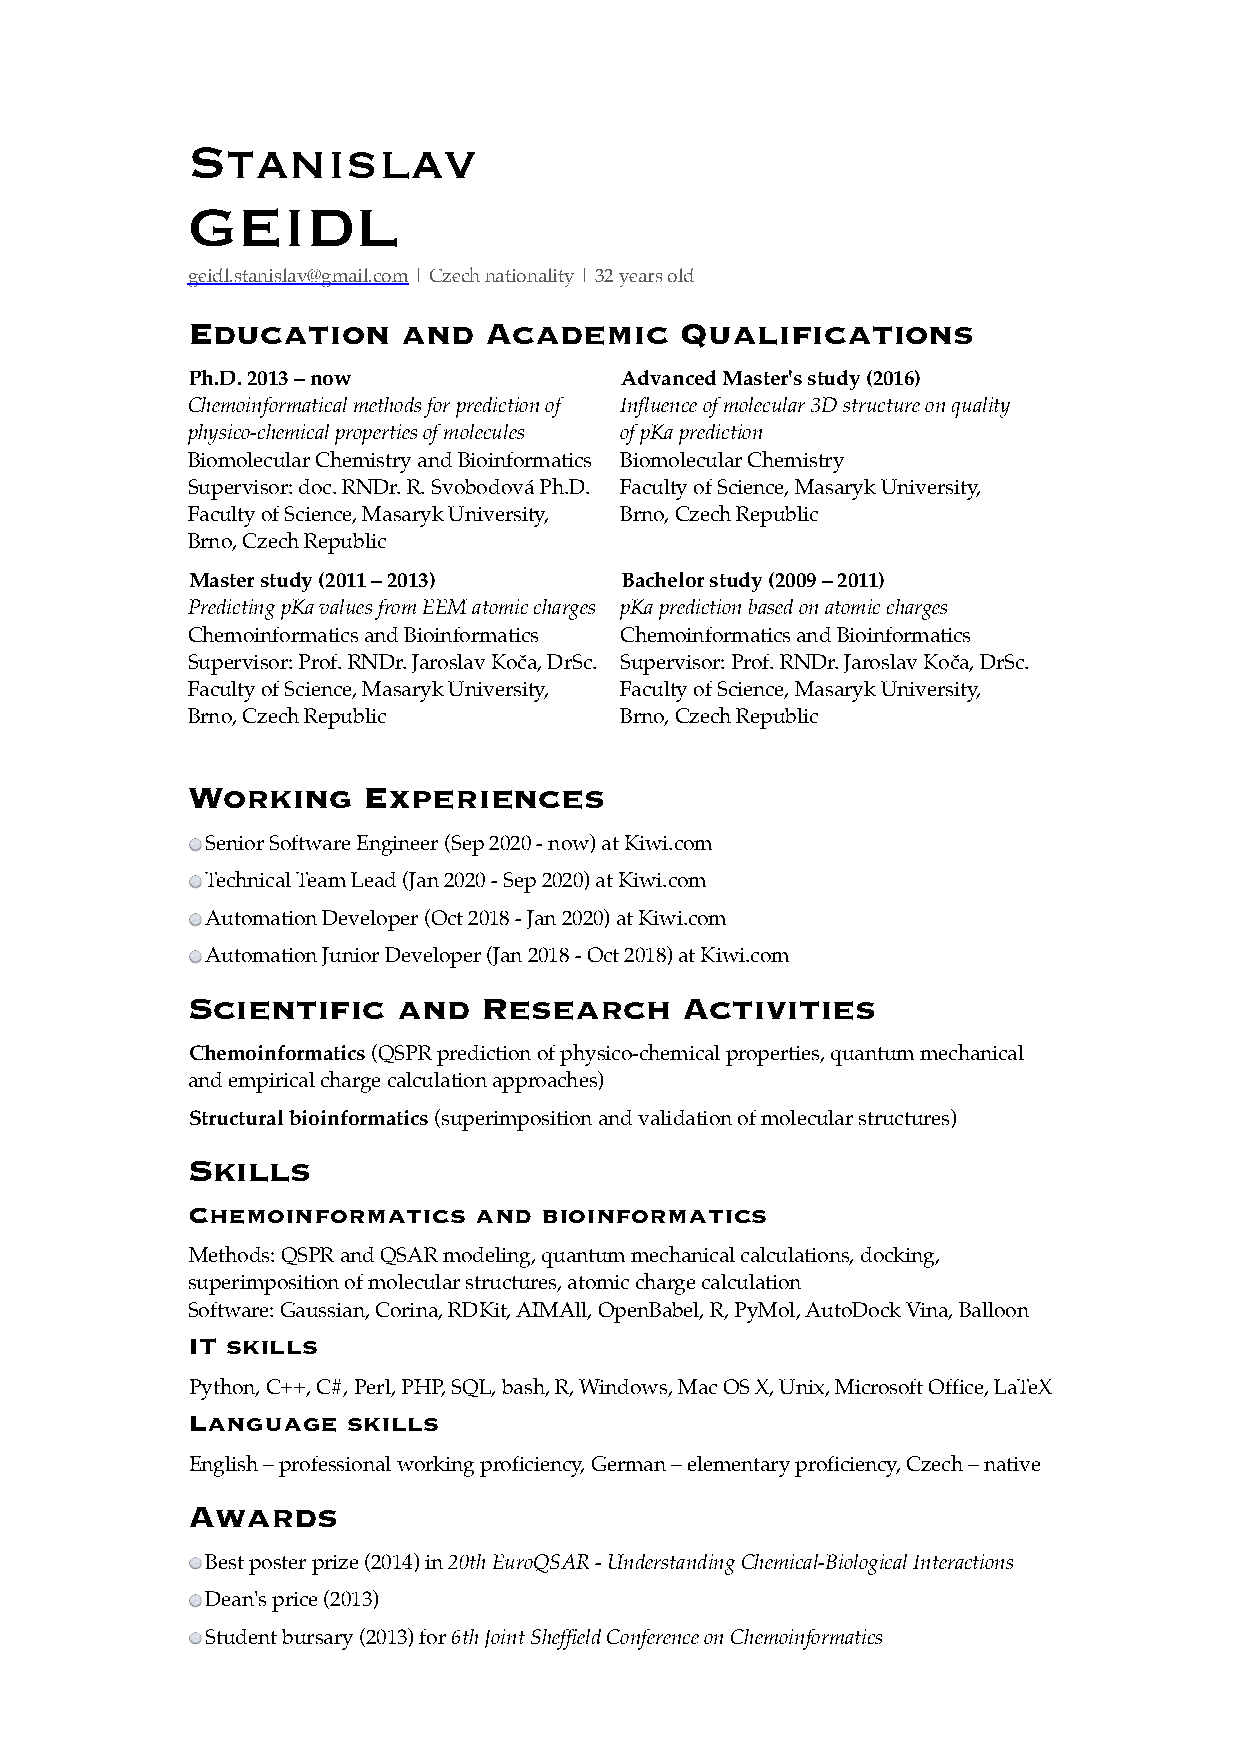
\includepdf[pages=-]{cv.pdf}


\clearpage

\thispagestyle{empty}
\null

\end{document}
